\section{\textbf{APPENDIX SKEWED-ASTROID CURVE}} \label{APPENDIX SKEWED-ASTROID CURVE}



\subsection       {Plot of SkwAstroid curve
	[\ref  {01-img-Plot of SkwAstroid curve.pdf} ] }
\label{ssec-01-img-Plot of SkwAstroid curve.pdf}

\subsection       {SkwAstroid Radius of Curvature
	[\ref      {02-img-SkwAstroid Radius of Curvature.pdf}] }
\label{ssec-02-img-SkwAstroid Radius of Curvature.pdf}

\subsection       {SkwAstroid Validation in LinuxCNC
	[\ref      {03-img-SkwAstroid-Validation-in-LinuxCNC.png} ] }
\label{ssec-03-img-SkwAstroid-Validation-in-LinuxCNC.png}

\subsection     {SkwAstroid Direction of Travel 3D
	[\ref      {04-img-SkwAstroid Direction of Travel 3D.pdf} ] }
\label{ssec-04-img-SkwAstroid Direction of Travel 3D.pdf}

\subsection       {SkwAstroid First and Second Order Taylors App
	[\ref      {05-img-SkwAstroid-First-and-Second-Order-Taylors-Approx.pdf}] }
\label{ssec-05-img-SkwAstroid-First-and-Second-Order-Taylors-Approx.pdf}

\subsection       {SkwAstroid First minus Second Order Taylors App
	[\ref      {06-img-SkwAstroid-First-minus-Second-Order-Taylors-Approx.pdf}] }
\label{ssec-06-img-SkwAstroid-First-minus-Second-Order-Taylors-Approx.pdf}

\subsection       {SkwAstroid Separate First Second Order Taylors App
	[\ref      {07-img-SkwAstroid-Separation-First-and-Second-Order-Taylors-Approx.pdf} ] }
\label{ssec-07-img-SkwAstroid-Separation-First-and-Second-Order-Taylors-Approx.pdf}

\subsection       {SkwAstroid Separation SAL and SCL
	[\ref      {08-img-SkwAstroid-Separation-SAL-and-SCL.pdf}] }
\label{ssec-08-img-SkwAstroid-Separation-SAL-and-SCL.pdf}

\subsection       {SkwAstroid Chord-error in close view 2 scales
	[\ref      {09-img-SkwAstroid-Chord-error-in-close-view-2-scales.pdf}] }
\label{ssec-09-img-SkwAstroid-Chord-error-in-close-view-2-scales.pdf}

\subsection       {SkwAstroid Four Components Feedrate Limit
	[\ref      {10-img-SkwAstroid-Four-Components-Feedrate-Limit.pdf} ] }
\label{ssec-10-img-SkwAstroid-Four-Components-Feedrate-Limit.pdf}

\subsection    {SkwAstroid FrateCommand FrateLimit and Curr-Frate
	[\ref      {11-img-SkwAstroid-FrateCommand-FrateLimit-and-Curr-Frate.pdf}] }
\label{ssec-11-img-SkwAstroid-FrateCommand-FrateLimit-and-Curr-Frate.pdf}

\subsection     {SkwAstroid FeedRateLimit minus CurrFeedRate
	[\ref      {12-img-SkwAstroid-FeedRateLimit-minus-CurrFeedRate.pdf} ] }
\label{ssec-12-img-SkwAstroid-FeedRateLimit-minus-CurrFeedRate.pdf}

\subsection     {SkwAstroid FC20-Nominal X and Y Feedrate Profiles
	[\ref      {13-img-SkwAstroid-FC20-Nominal-X-and-Y-Feedrate-Profiles.pdf} ] }
\label{ssec-13-img-SkwAstroid-FC20-Nominal-X-and-Y-Feedrate-Profiles.pdf}

\subsection     {SkwAstroid FC20 Nominal Tangential Acceleration
	[\ref      {14-img-SkwAstroid-FC20-Nominal-Tangential-Acceleration.pdf} ] }
\label{ssec-14-img-SkwAstroid-FC20-Nominal-Tangential-Acceleration.pdf}

\subsection     {SkwAstroid FC20 Nominal Rising S-Curve Profile
	[\ref      {15-img-SkwAstroid-FC20-Nominal-Rising-S-Curve-Profile.pdf} ] }
\label{ssec-15-img-SkwAstroid-FC20-Nominal-Rising-S-Curve-Profile.pdf}

\subsection     {SkwAstroid FC20 Nominal Falling S-Curve Profile
	[\ref      {16-img-SkwAstroid-FC20-Nominal-Falling-S-Curve-Profile.pdf}] }
\label{ssec-16-img-SkwAstroid-FC20-Nominal-Falling-S-Curve-Profile.pdf}

\subsection       {SkwAstroid FC10 Colored Feedrate Profile ngcode
	[\ref      {17-img-SkwAstroid-FC10-Colored-Feedrate-Profile-data_ngcode.png} ] }
\label{ssec-17-img-SkwAstroid-FC10-Colored-Feedrate-Profile-data_ngcode.png}

\subsection       {SkwAstroid FC20 Colored Feedrate Profile ngcode
	[\ref      {18-img-SkwAstroid-FC20-Colored-Feedrate-Profile-data_ngcode.png} ] }
\label{ssec-18-img-SkwAstroid-FC20-Colored-Feedrate-Profile-data_ngcode.png}

Continue ...\\

\subsection       {SkwAstroid FC30 Colored Feedrate Profile ngcode
	[\ref      {19-img-SkwAstroid-FC30-Colored-Feedrate-Profile-data_ngcode.png} ] }
\label{ssec-19-img-SkwAstroid-FC30-Colored-Feedrate-Profile-data_ngcode.png}

\subsection       {SkwAstroid FC40 Colored Feedrate Profile ngcode
	[\ref      {20-img-SkwAstroid-FC40-Colored-Feedrate-Profile-data_ngcode.png} ] }
\label{ssec-20-img-SkwAstroid-FC40-Colored-Feedrate-Profile-data_ngcode.png}

\subsection       {SkwAstroid FC10 Tangential Acceleration
	[\ref      {21-img-SkwAstroid-FC10-Tangential-Acceleration.pdf}] }
\label{ssec-21-img-SkwAstroid-FC10-Tangential-Acceleration.pdf}

\subsection       {SkwAstroid FC20 Tangential Acceleration
	[\ref      {22-img-SkwAstroid-FC20-Tangential-Acceleration.pdf}] }
\label{ssec-22-img-SkwAstroid-FC20-Tangential-Acceleration.pdf}

\subsection       {SkwAstroid FC30 Tangential Acceleration
	[\ref      {23-img-SkwAstroid-FC30-Tangential-Acceleration.pdf}] }
\label{ssec-23-img-SkwAstroid-FC30-Tangential-Acceleration.pdf}

\subsection       {SkwAstroid FC40 Tangential Acceleration
	[\ref      {24-img-SkwAstroid-FC40-Tangential-Acceleration.pdf}] }
\label{ssec-24-img-SkwAstroid-FC40-Tangential-Acceleration.pdf}

\subsection       {SkwAstroid FC20 Nominal Separation NAL and NCL
	[\ref      {25-img-SkwAstroid-FC20-Nominal-Separation-NAL-and-NCL.pdf}] }
\label{ssec-25-img-SkwAstroid-FC20-Nominal-Separation-NAL-and-NCL.pdf}

\subsection       {SkwAstroid SAL minus SCL for FC10 FC20 FC30 FC40
	[\ref      {26-img-SkwAstroid-Difference-SAL-minus-SCL-for-FC10-FC20-FC30-FC40.pdf}] }
\label{ssec-26-img-SkwAstroid-Difference-SAL-minus-SCL-for-FC10-FC20-FC30-FC40.pdf}


\subsection       {SkwAstroid FC10 FrateCmd CurrFrate X-Frate Y-Frate
	[\ref      {27-img-SkwAstroid-FC10-FrateCmd-CurrFrate-X-Frate-Y-Frate.pdf}] }
\label{ssec-27-img-SkwAstroid-FC10-FrateCmd-CurrFrate-X-Frate-Y-Frate.pdf}

\subsection       {SkwAstroid FC20 FrateCmd CurrFrate X-Frate Y-Frate
	[\ref      {28-img-SkwAstroid-FC20-FrateCmd-CurrFrate-X-Frate-Y-Frate.pdf}] }
\label{ssec-28-img-SkwAstroid-FC20-FrateCmd-CurrFrate-X-Frate-Y-Frate.pdf}

\subsection       {SkwAstroid FC30 FrateCmd CurrFrate X-Frate Y-Frate
	[\ref      {29-img-SkwAstroid-FC30-FrateCmd-CurrFrate-X-Frate-Y-Frate.pdf}] }
\label{ssec-29-img-SkwAstroid-FC30-FrateCmd-CurrFrate-X-Frate-Y-Frate.pdf}

\subsection       {SkwAstroid FC40 FrateCmd CurrFrate X-Frate Y-Frate
	[\ref      {30-img-SkwAstroid-FC40-FrateCmd-CurrFrate-X-Frate-Y-Frate.pdf}] }
\label{ssec-30-img-SkwAstroid-FC40-FrateCmd-CurrFrate-X-Frate-Y-Frate.pdf}

\subsection       {SkwAstroid FC10 Four Components FeedrateLimit
	[\ref      {31-img-SkwAstroid-FC10-Four-Components-FeedrateLimit.pdf}] }
\label{ssec-31-img-SkwAstroid-FC10-Four-Components-FeedrateLimit.pdf}

\subsection       {SkwAstroid FC20 Four Components FeedrateLimit
	[\ref      {32-img-SkwAstroid-FC20-Four-Components-FeedrateLimit.pdf}] }
\label{ssec-32-img-SkwAstroid-FC20-Four-Components-FeedrateLimit.pdf}

\subsection       {SkwAstroid FC30 Four Components FeedrateLimit
	[\ref      {33-img-SkwAstroid-FC30-Four-Components-FeedrateLimit.pdf}] }
\label{ssec-33-img-SkwAstroid-FC30-Four-Components-FeedrateLimit.pdf}

\subsection       {SkwAstroid FC40 Four Components FeedrateLimit
	[\ref      {34-img-SkwAstroid-FC40-Four-Components-FeedrateLimit.pdf}]}
\label{ssec-34-img-SkwAstroid-FC40-Four-Components-FeedrateLimit.pdf}

\subsection       {SkwAstroid Histogram Points FC10 FC20 FC30 FC40
	[\ref      {35-img-SkwAstroid-Histogram-Points-FC10-FC20-FC30-FC40.pdf}] }
\label{ssec-35-img-SkwAstroid-Histogram-Points-FC10-FC20-FC30-FC40.pdf}

\subsection    {SkwAstroid Table distribution of interpolated points
	[\ref      {tab-SkwAstroid Table distribution of interpolated points}] }
\label{ssec-tab-SkwAstroid Table distribution of interpolated points}

\subsection         {SkwAstroid Table FC10-20-30-40 Run Performance data
	[\ref      {tab-app4-SkwAstroid-Table-FC10-20-30-40-Run-Performance-data}] }
\label{ssec-tab-app4-SkwAstroid-Table-FC10-20-30-40-Run-Performance-data}


%% =====================================================
%% =====================================================
\clearpage
\pagebreak

\begin{figure}
	\caption     {Plot of SkwAstroid curve}
	\label{01-img-Plot of SkwAstroid curve.pdf}
	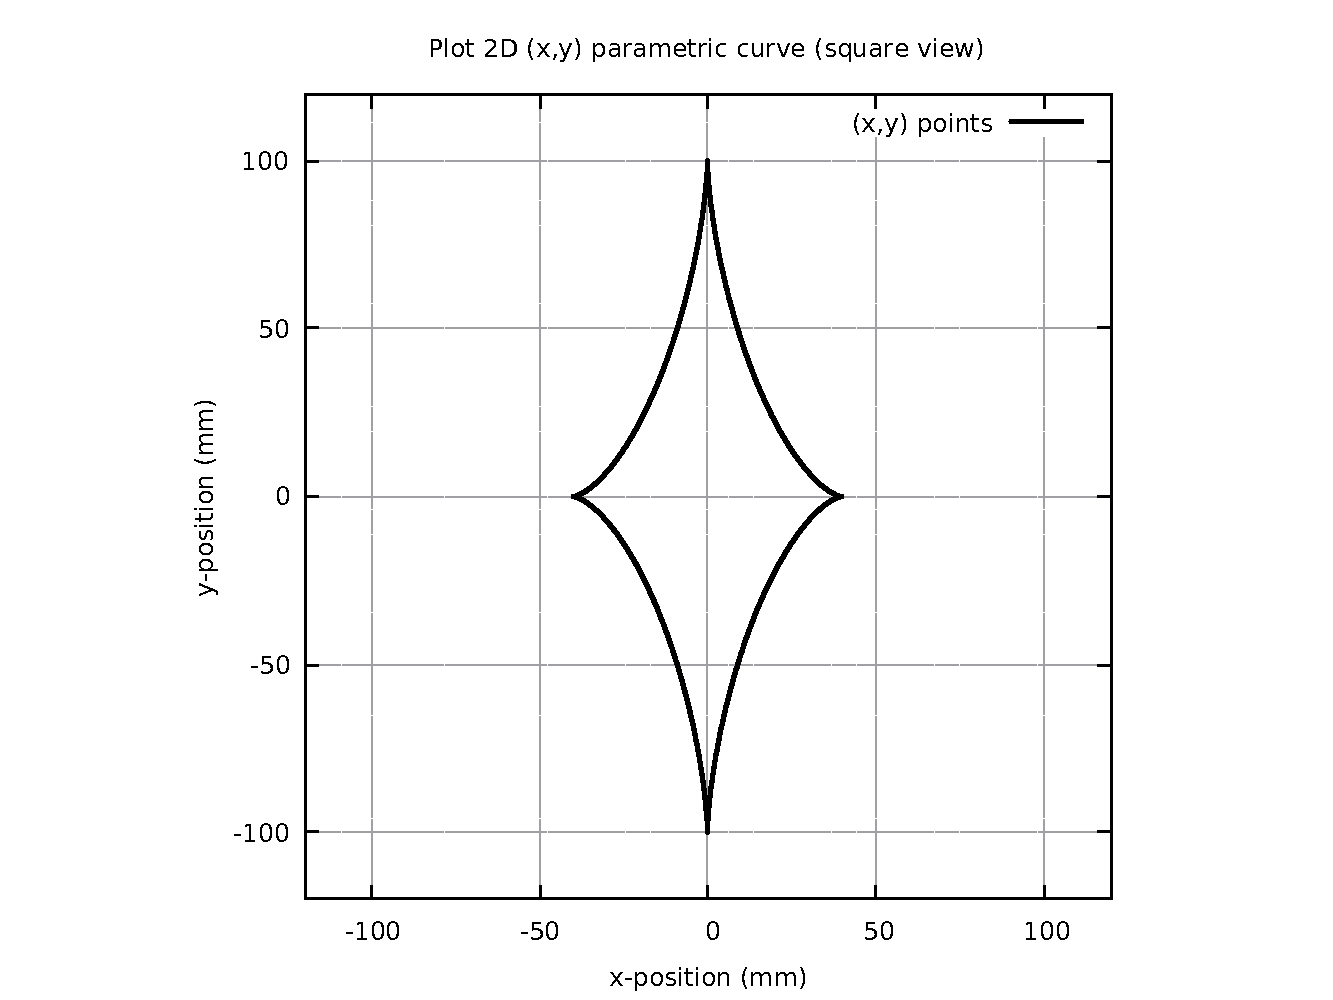
\includegraphics[width=1.00\textwidth]{Chap4/appendix/app-SkwAstroid/plots/01-img-Plot of SkwAstroid curve.pdf}
\end{figure}	


\begin{figure}
	\caption     {SkwAstroid Radius of Curvature}
	\label{02-img-SkwAstroid Radius of Curvature.pdf}
	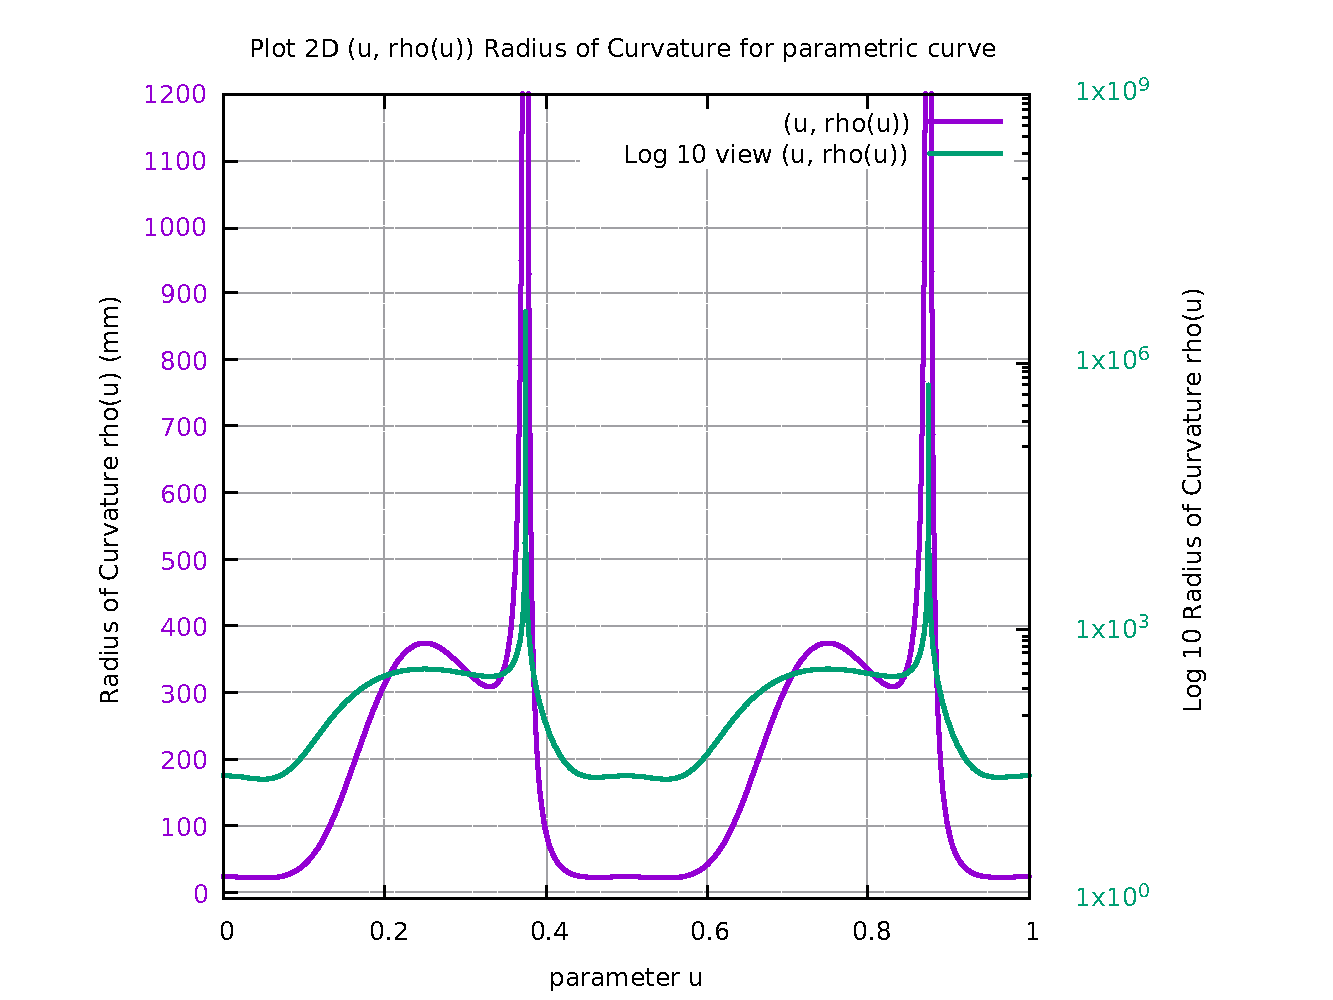
\includegraphics[width=1.00\textwidth]{Chap4/appendix/app-SkwAstroid/plots/02-img-SkwAstroid Radius of Curvature.pdf} 
\end{figure}	


%% ==================================================
\clearpage
\pagebreak

\begin{figure}
	\caption     {SkwAstroid Validation in LinuxCNC}
	\label{03-img-SkwAstroid-Validation-in-LinuxCNC.png}
	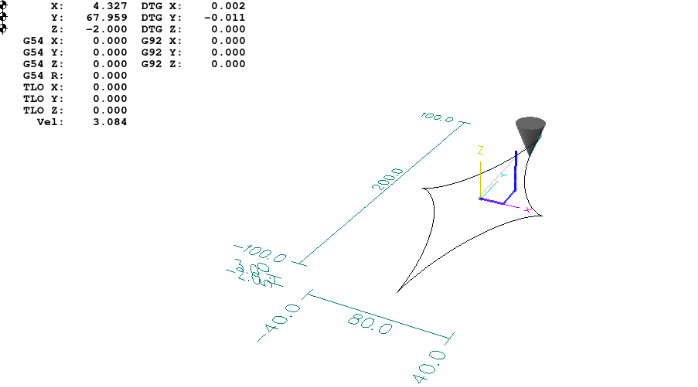
\includegraphics[width=1.00\textwidth]{Chap4/appendix/app-SkwAstroid/plots/03-img-SkwAstroid-Validation-in-LinuxCNC.png}
\end{figure}


\begin{figure}
	\caption     {SkwAstroid Direction of Travel 3D}
	\label{04-img-SkwAstroid Direction of Travel 3D.pdf}
	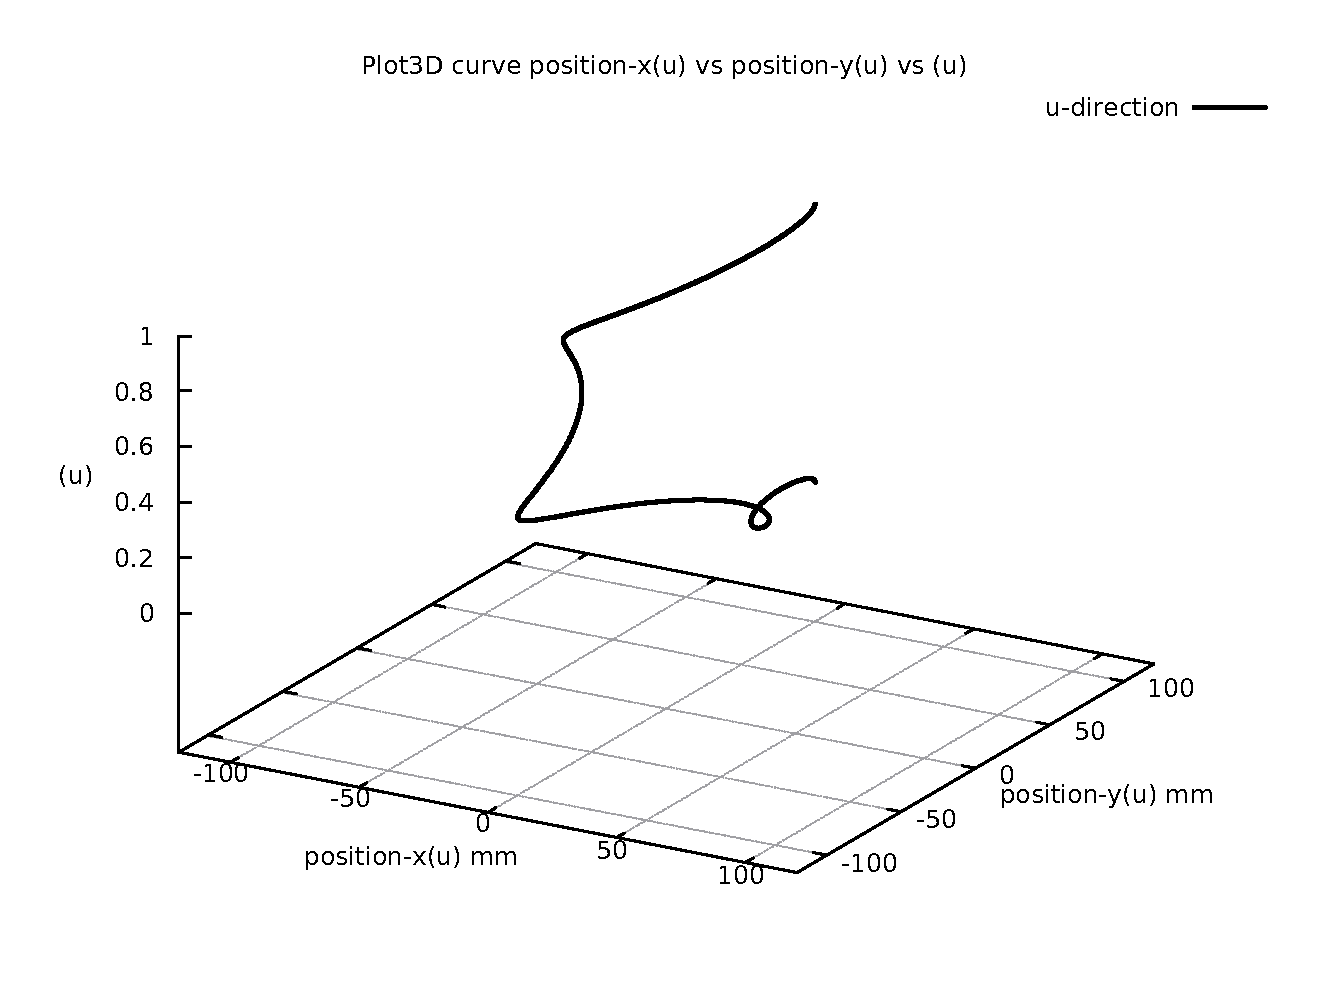
\includegraphics[width=1.00\textwidth]{Chap4/appendix/app-SkwAstroid/plots/04-img-SkwAstroid Direction of Travel 3D.pdf}
\end{figure}

%% ==================================================
\clearpage
\pagebreak

\begin{figure}
	\caption     {SkwAstroid First and Second Order Taylor's Approximation}
	\label{05-img-SkwAstroid-First-and-Second-Order-Taylors-Approx.pdf}
	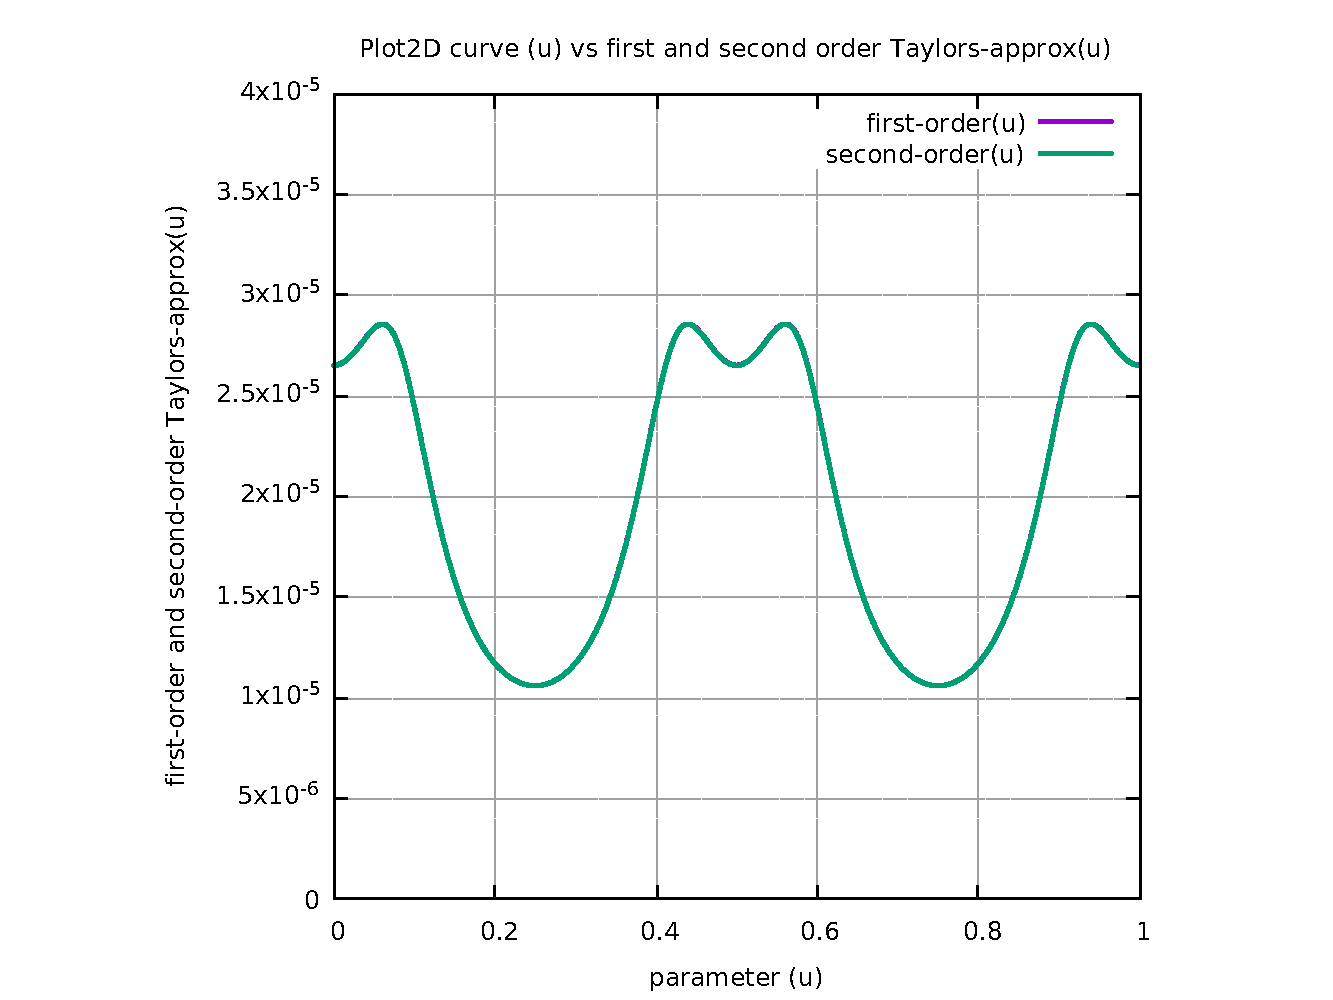
\includegraphics[width=1.00\textwidth]{Chap4/appendix/app-SkwAstroid/plots/05-img-SkwAstroid-First-and-Second-Order-Taylors-Approx.pdf}
\end{figure}


\begin{figure}
	\caption     {SkwAstroid First minus Second Order Taylor's Approximation}
	\label{06-img-SkwAstroid-First-minus-Second-Order-Taylors-Approx.pdf}
	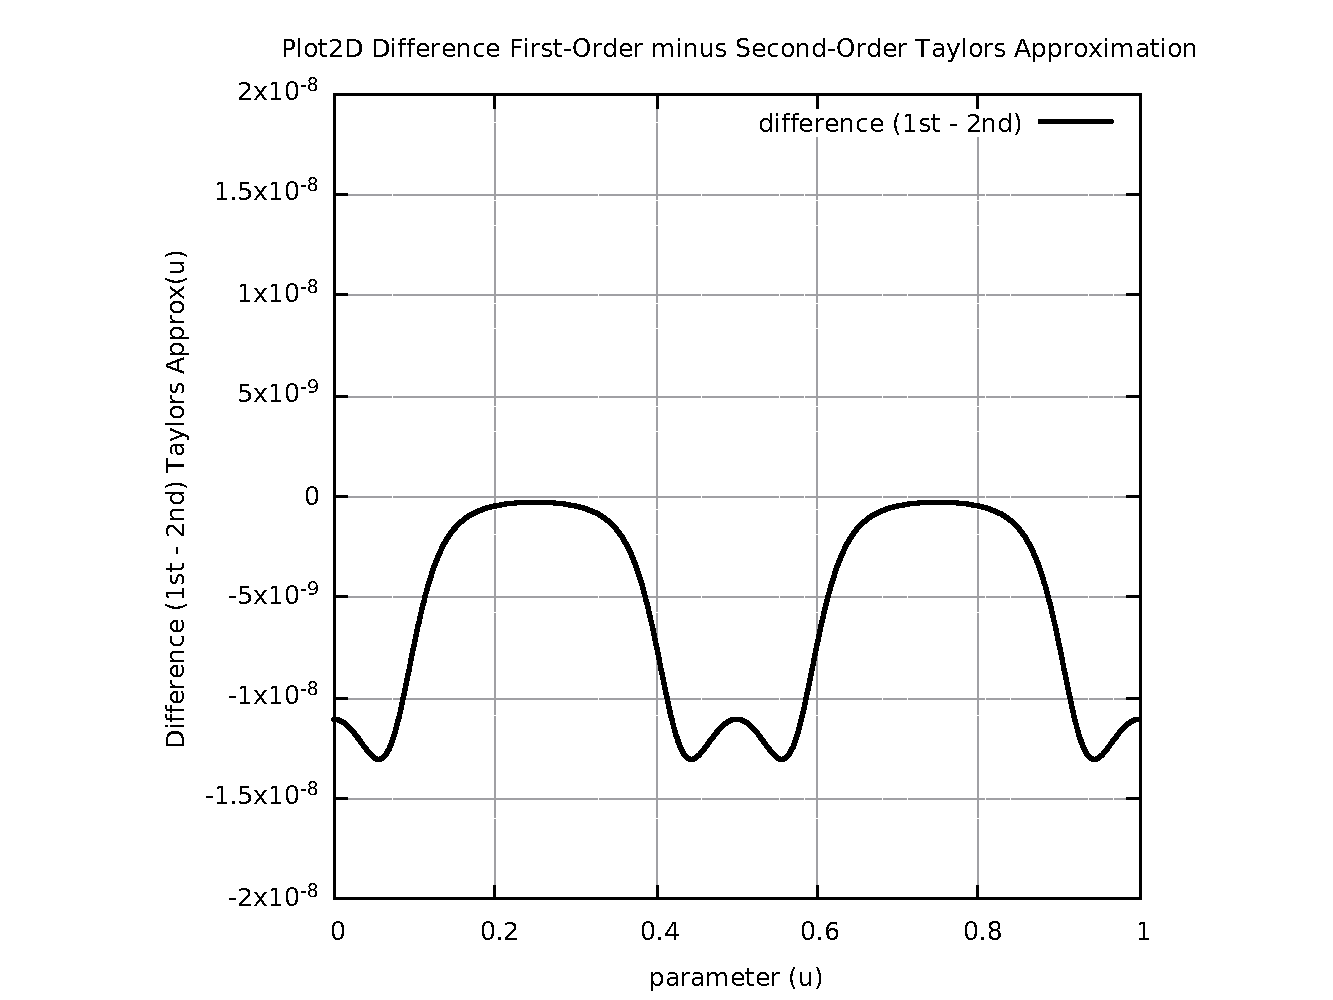
\includegraphics[width=1.00\textwidth]{Chap4/appendix/app-SkwAstroid/plots/06-img-SkwAstroid-First-minus-Second-Order-Taylors-Approx.pdf}
\end{figure}

%% ==================================================
\clearpage
\pagebreak

\begin{figure}
	\caption     {SkwAstroid Separation First and Second Order Taylor's Approximation}
	\label{07-img-SkwAstroid-Separation-First-and-Second-Order-Taylors-Approx.pdf}
	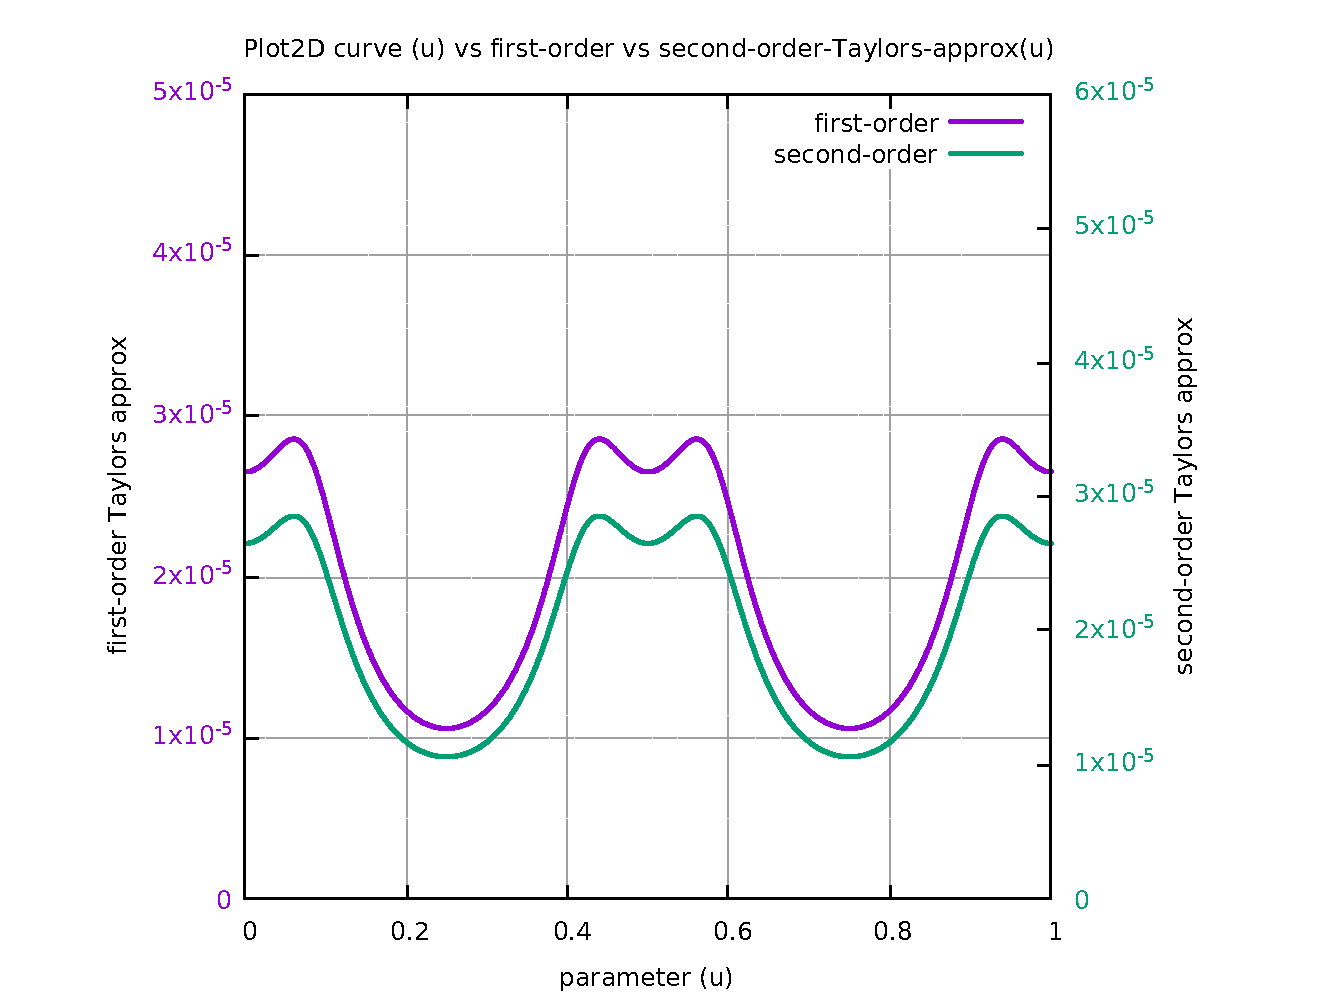
\includegraphics[width=1.00\textwidth]{Chap4/appendix/app-SkwAstroid/plots/07-img-SkwAstroid-First-and-Second-Order-Taylors-Approx.pdf}
\end{figure}


\begin{figure}
	\caption     {SkwAstroid Separation SAL and SCL}
	\label{08-img-SkwAstroid-Separation-SAL-and-SCL.pdf}
	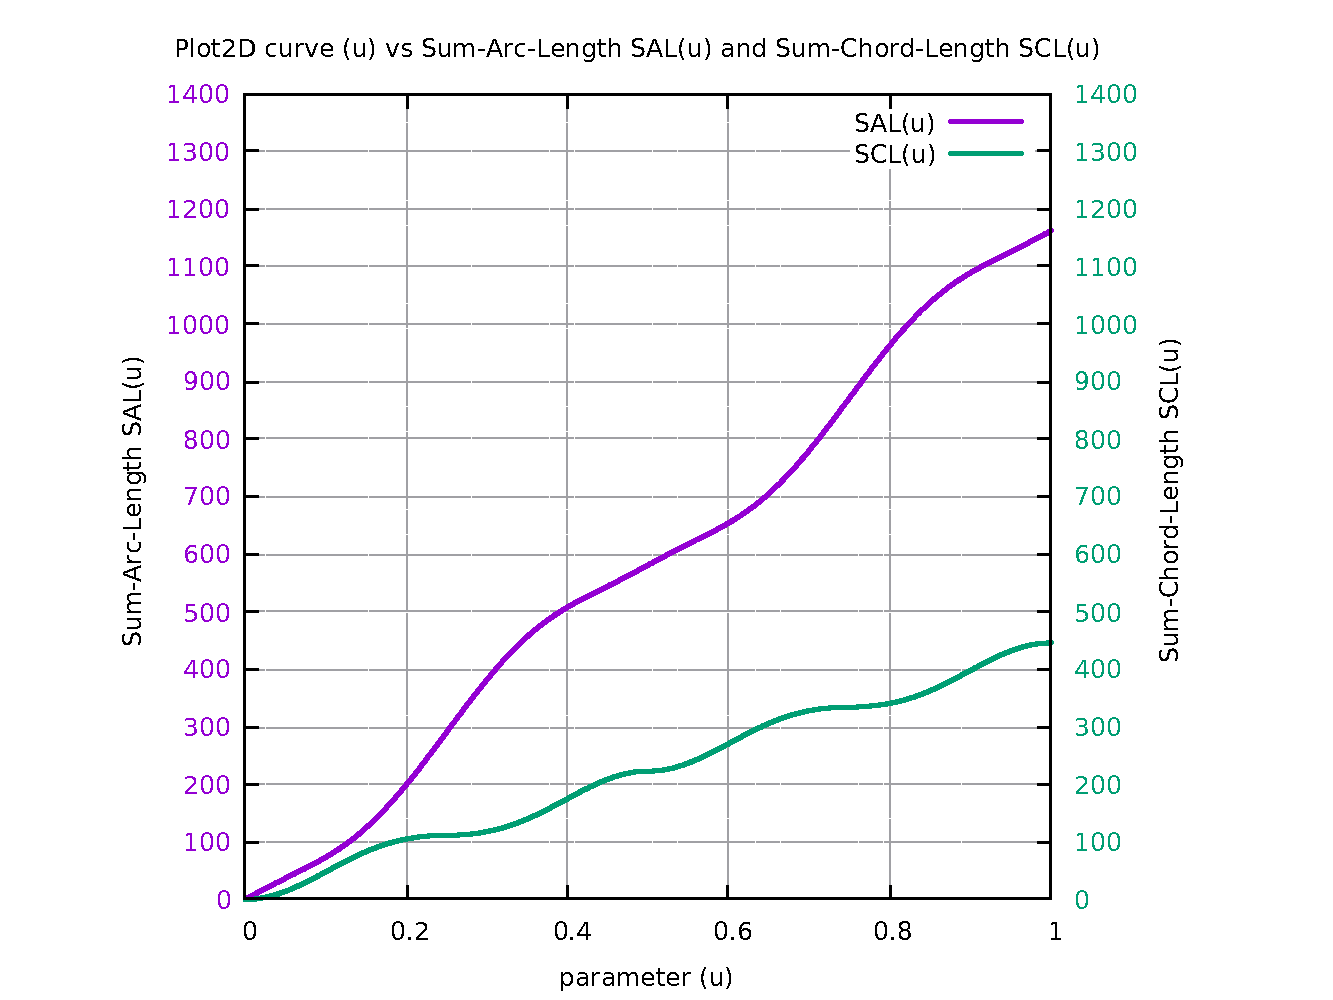
\includegraphics[width=1.00\textwidth]{Chap4/appendix/app-SkwAstroid/plots/08-img-SkwAstroid-Separation-SAL-and-SCL.pdf}
\end{figure}

%% ==================================================
\clearpage
\pagebreak

\begin{figure}
	\caption     {SkwAstroid Chord-error in close view 2 scales}
	\label{09-img-SkwAstroid-Chord-error-in-close-view-2-scales.pdf}
	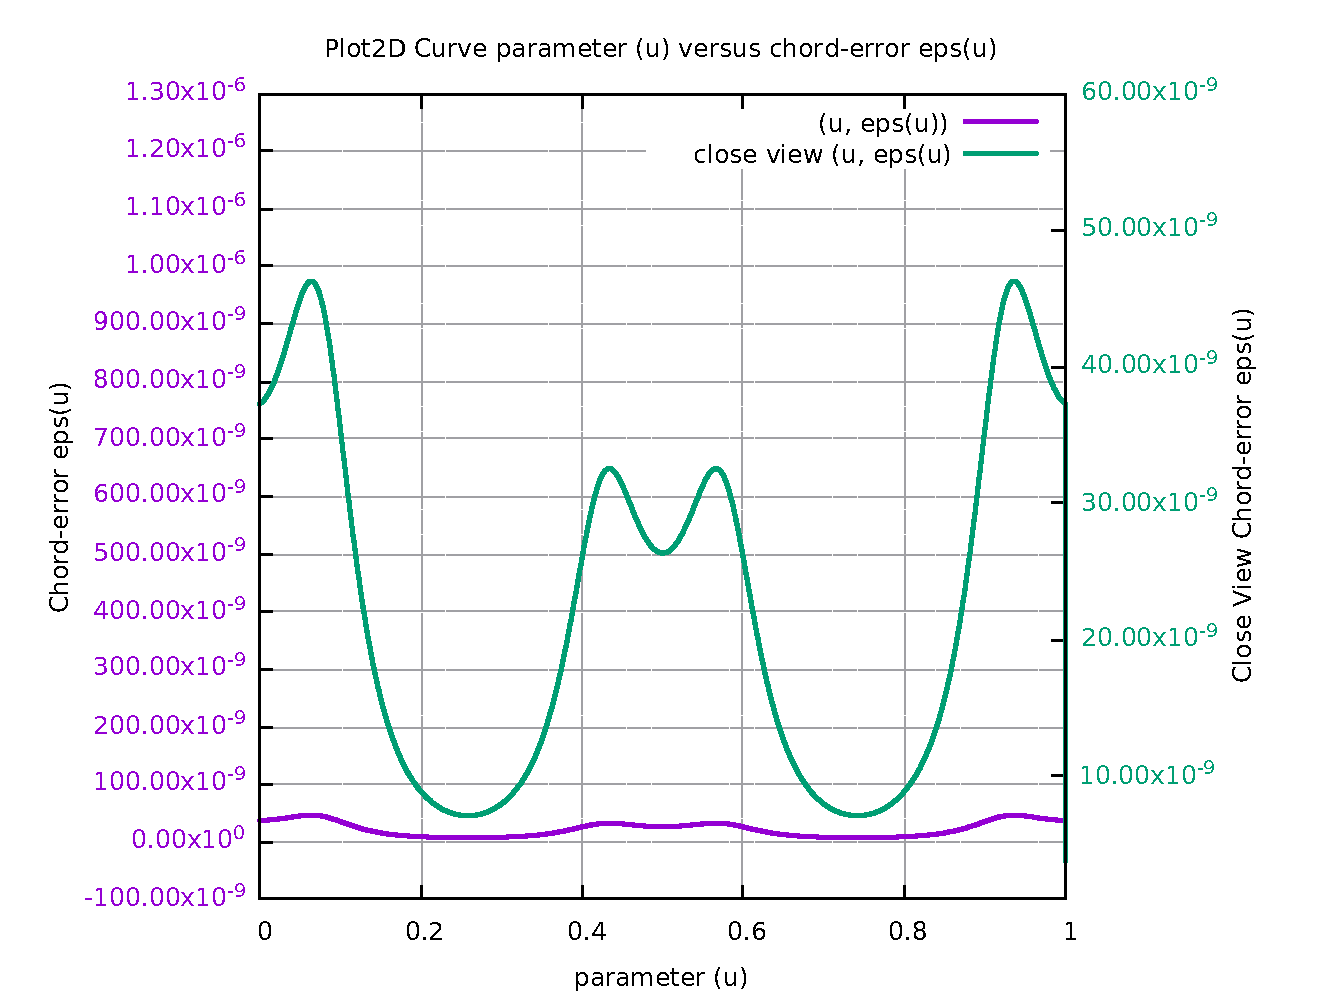
\includegraphics[width=1.00\textwidth]{Chap4/appendix/app-SkwAstroid/plots/09-img-SkwAstroid-Chord-error-in-close-view-2-scales.pdf}
\end{figure}

\begin{figure}
	\caption     {SkwAstroid Four Components Feedrate Limit}
	\label{10-img-SkwAstroid-Four-Components-Feedrate-Limit.pdf}
	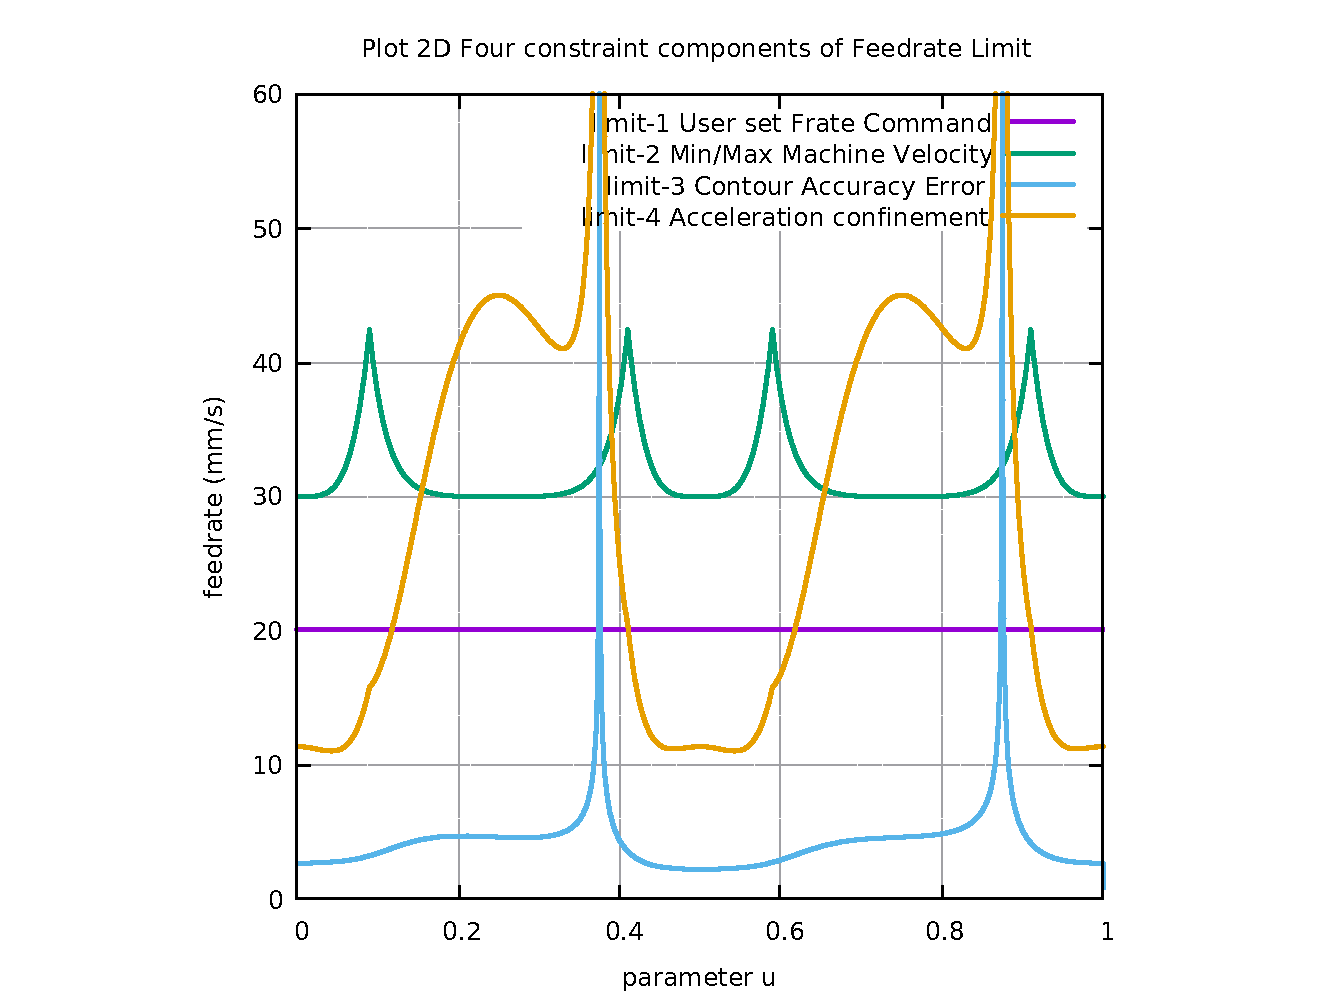
\includegraphics[width=1.00\textwidth]{Chap4/appendix/app-SkwAstroid/plots/10-img-SkwAstroid-Four-Components-Feedrate-Limit.pdf}
\end{figure}

%% ==================================================
\clearpage
\pagebreak

\begin{figure}
	\caption     {SkwAstroid FrateCommand FrateLimit and Curr-Frate}
	\label{11-img-SkwAstroid-FrateCommand-FrateLimit-and-Curr-Frate.pdf}
	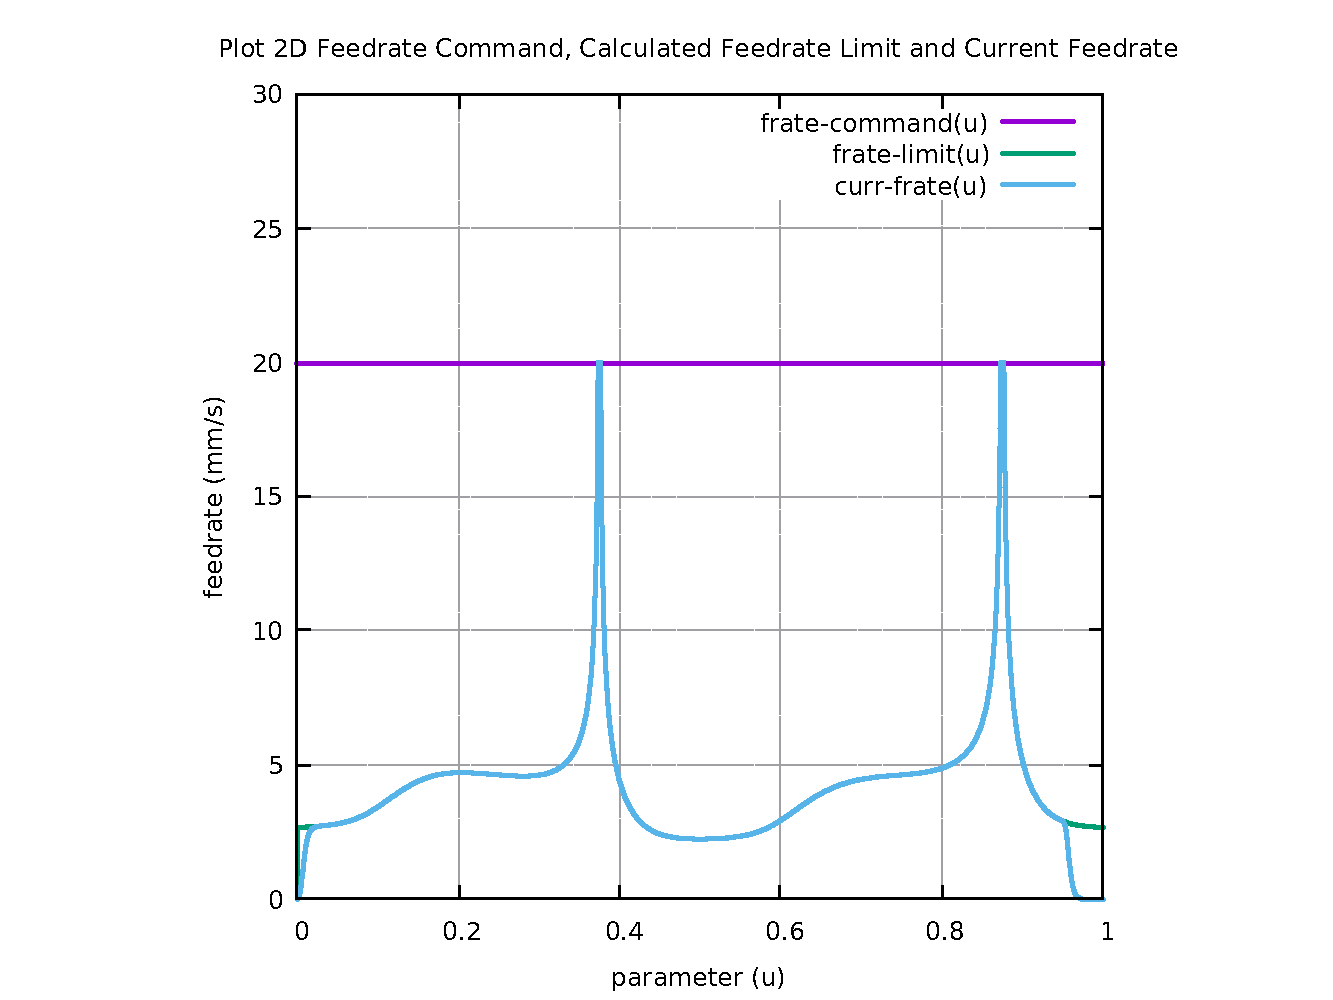
\includegraphics[width=1.00\textwidth]{Chap4/appendix/app-SkwAstroid/plots/11-img-SkwAstroid-FrateCommand-FrateLimit-and-Curr-Frate.pdf}
\end{figure}

\begin{figure}
	\caption     {SkwAstroid FeedRateLimit minus CurrFeedRate}
	\label{12-img-SkwAstroid-FeedRateLimit-minus-CurrFeedRate.pdf}
	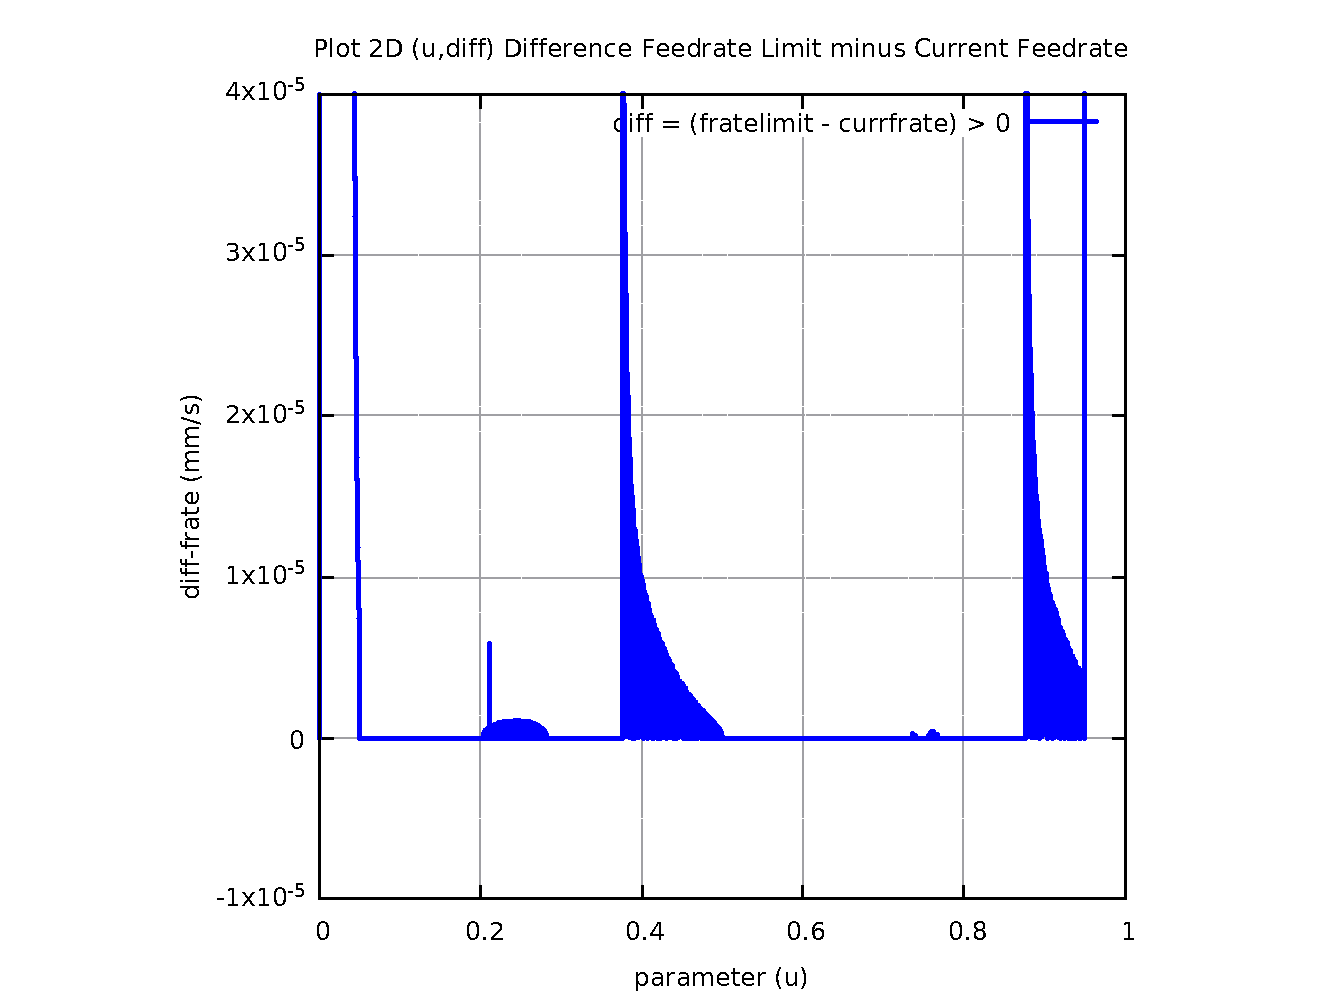
\includegraphics[width=1.00\textwidth]{Chap4/appendix/app-SkwAstroid/plots/12-img-SkwAstroid-FeedRateLimit-minus-CurrFeedRate.pdf}
\end{figure}

%% ==================================================
\clearpage
\pagebreak

\begin{figure}
	\caption     {SkwAstroid FC20-Nominal X and Y Feedrate Profiles}
	\label{13-img-SkwAstroid-FC20-Nominal-X-and-Y-Feedrate-Profiles.pdf}
	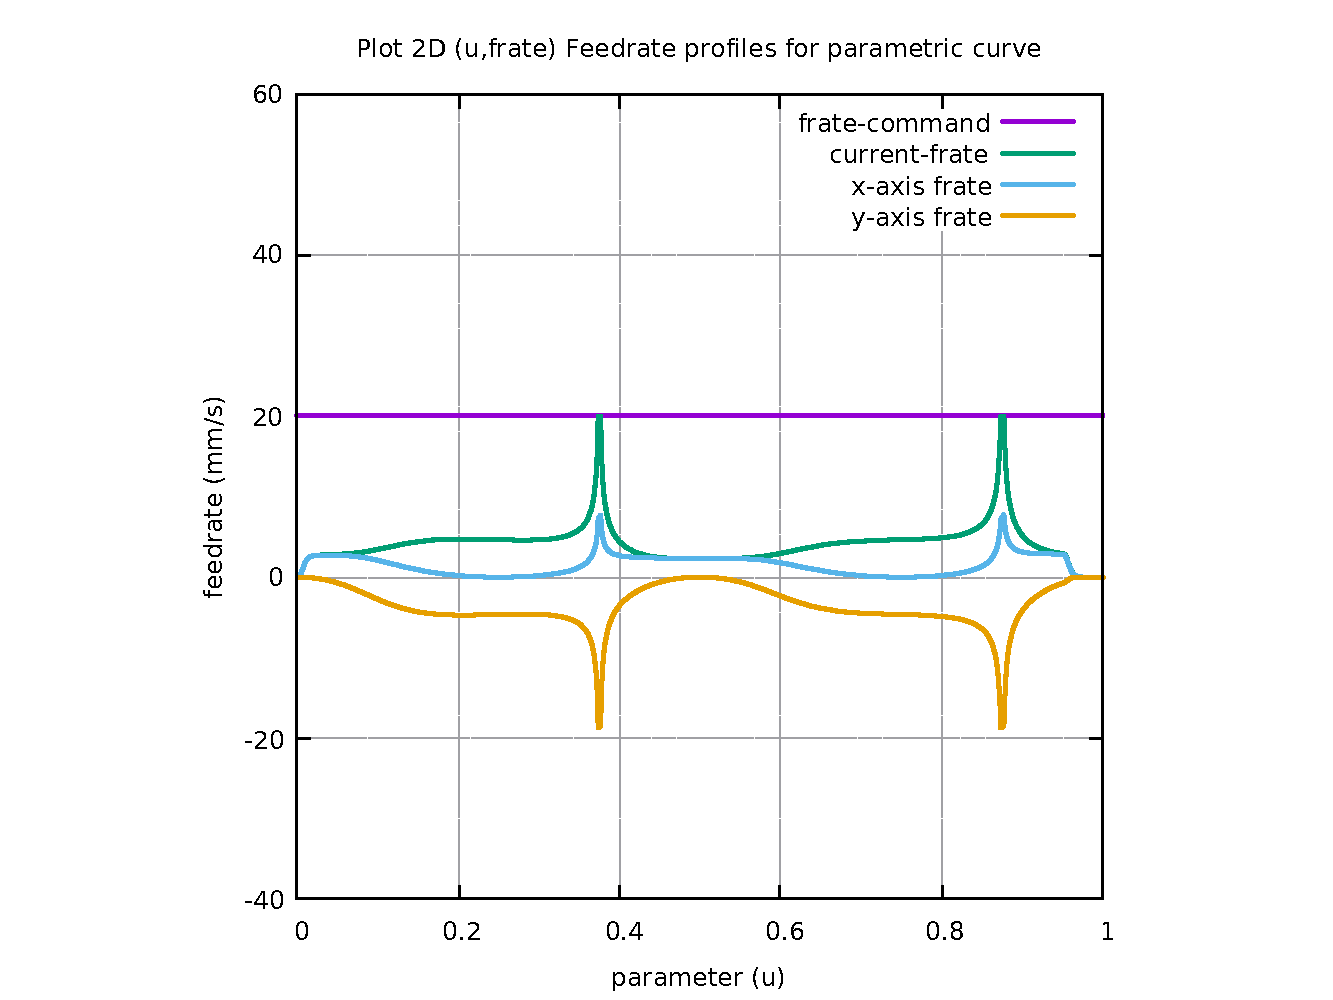
\includegraphics[width=1.00\textwidth]{Chap4/appendix/app-SkwAstroid/plots/13-img-SkwAstroid-FC20-Nominal-X-and-Y-Feedrate-Profiles.pdf}
\end{figure}


\begin{figure}
	\caption     {SkwAstroid FC20 Nominal Tangential Acceleration}
	\label{14-img-SkwAstroid-FC20-Nominal-Tangential-Acceleration.pdf}
	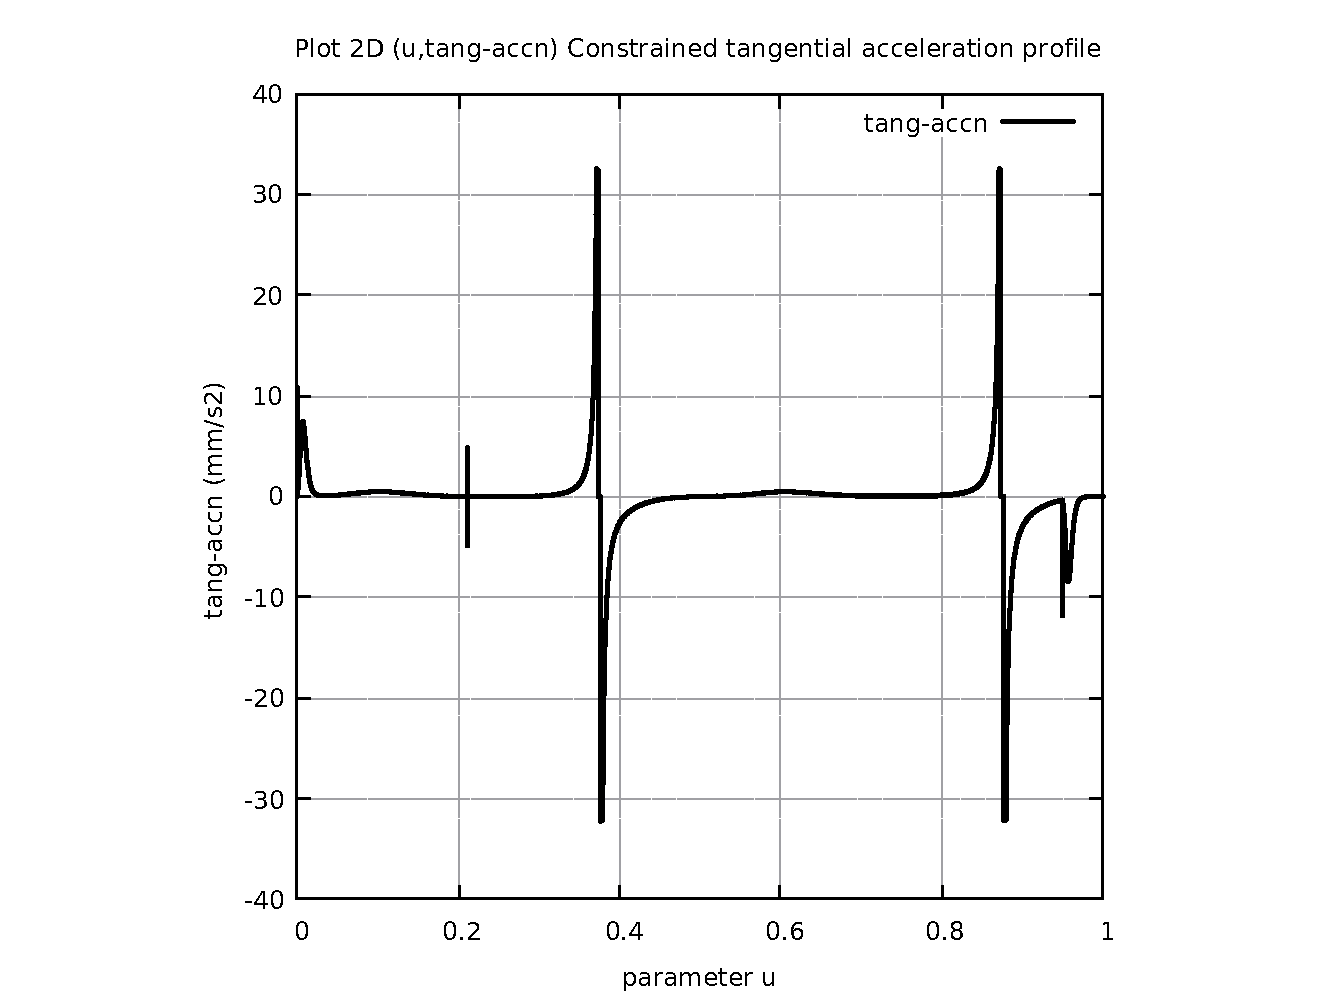
\includegraphics[width=1.00\textwidth]{Chap4/appendix/app-SkwAstroid/plots/14-img-SkwAstroid-FC20-Nominal-Tangential-Acceleration.pdf}
\end{figure}

%% ==================================================
\clearpage
\pagebreak

\begin{figure}
	\caption     {SkwAstroid FC20 Nominal Rising S-Curve Profile}
	\label{15-img-SkwAstroid-FC20-Nominal-Rising-S-Curve-Profile.pdf}
	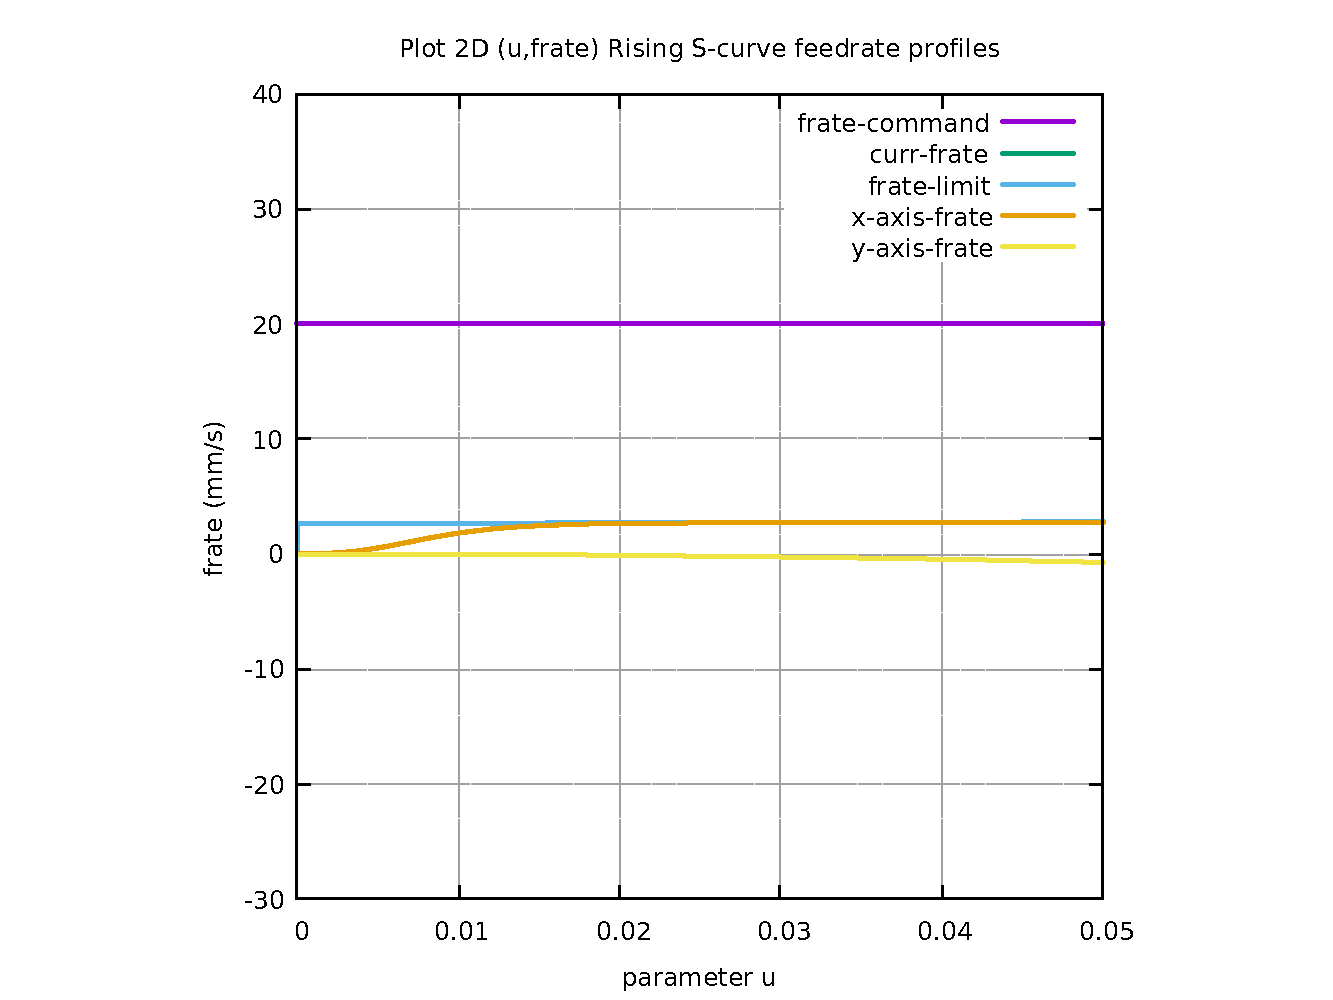
\includegraphics[width=1.00\textwidth]{Chap4/appendix/app-SkwAstroid/plots/15-img-SkwAstroid-FC20-Nominal-Rising-S-Curve-Profile.pdf}
\end{figure}


\begin{figure}
	\caption     {SkwAstroid FC20 Nominal Falling S-Curve Profile}
	\label{16-img-SkwAstroid-FC20-Nominal-Falling-S-Curve-Profile.pdf}
	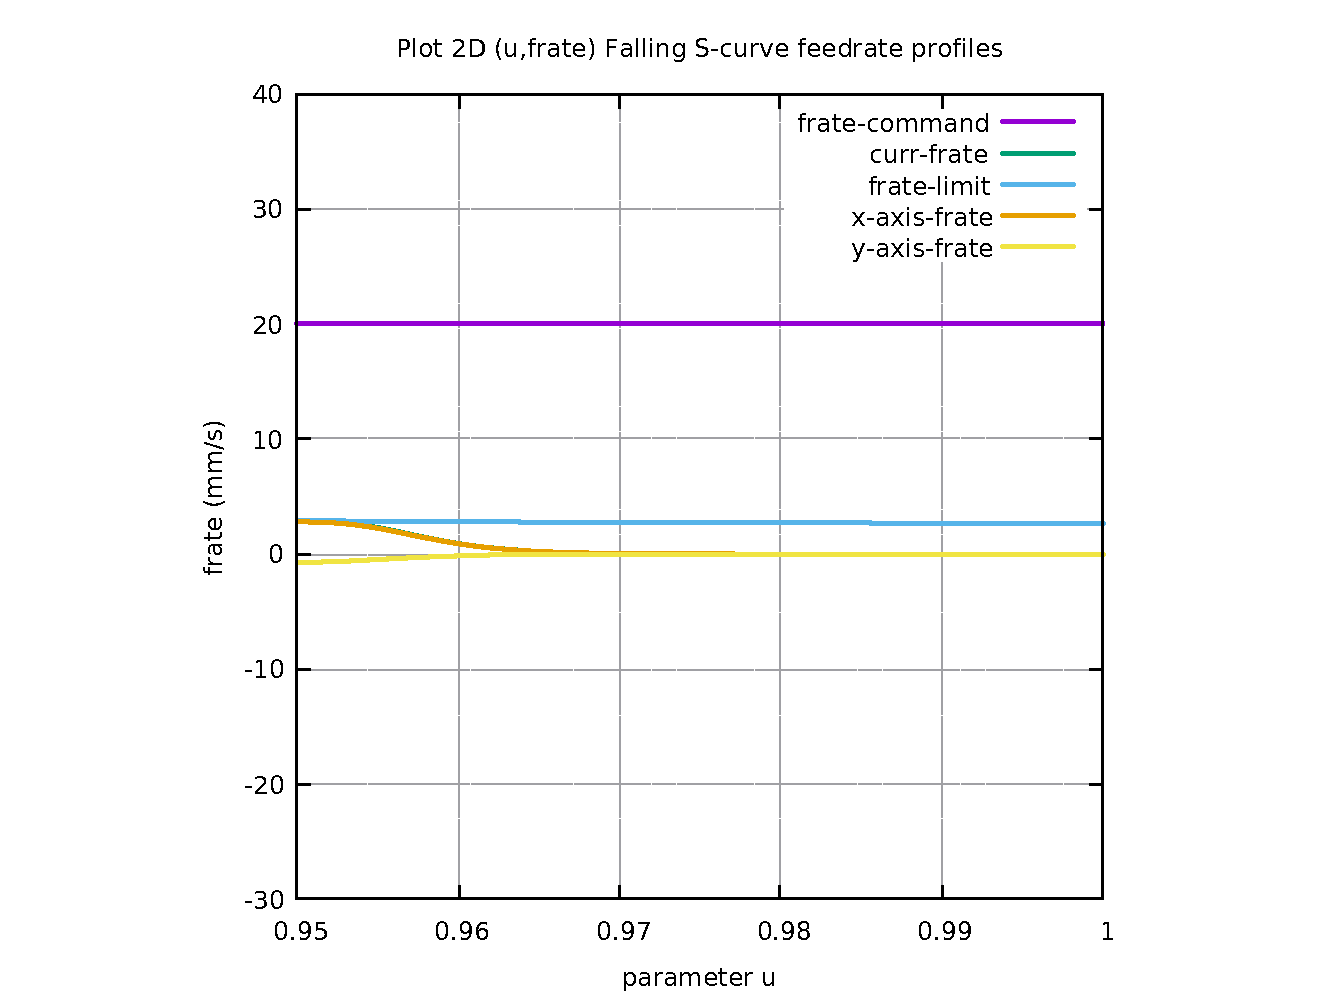
\includegraphics[width=1.00\textwidth]{Chap4/appendix/app-SkwAstroid/plots/16-img-SkwAstroid-FC20-Nominal-Falling-S-Curve-Profile.pdf}
\end{figure}

%% ==================================================
\clearpage
\pagebreak

\begin{figure}
	\caption     {SkwAstroid FC10 Colored Feedrate Profile data ngcode}
	\label{17-img-SkwAstroid-FC10-Colored-Feedrate-Profile-data_ngcode.png}
	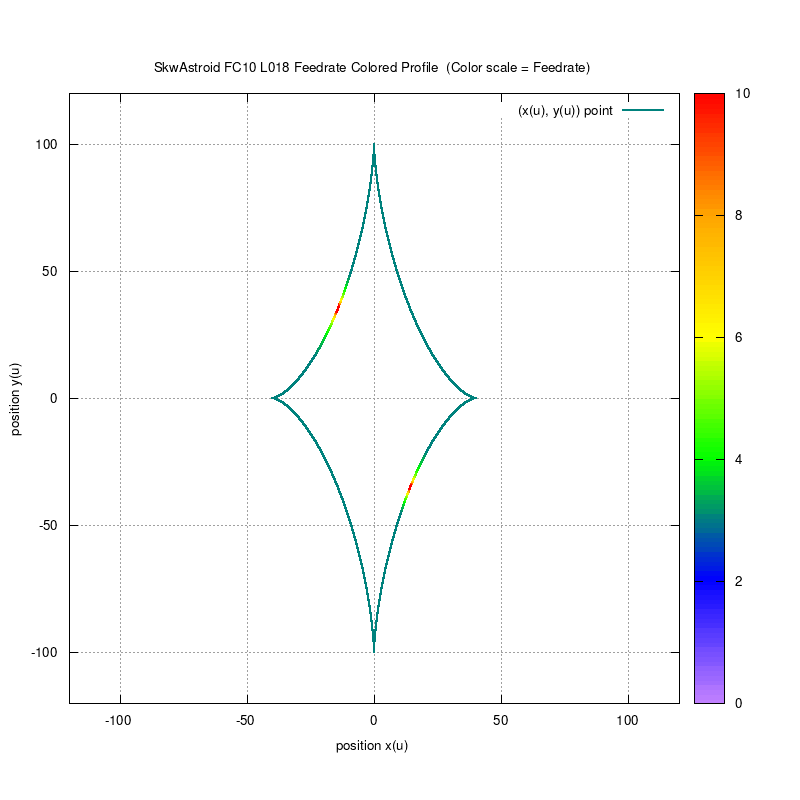
\includegraphics[width=0.75\textwidth]{Chap4/appendix/app-SkwAstroid/plots/17-img-SkwAstroid-FC10-Colored-Feedrate-Profile-data_ngcode.png}
\end{figure}


\begin{figure}
	\caption     {SkwAstroid FC20 Colored Feedrate Profile data ngcode}
	\label{18-img-SkwAstroid-FC20-Colored-Feedrate-Profile-data_ngcode.png}
	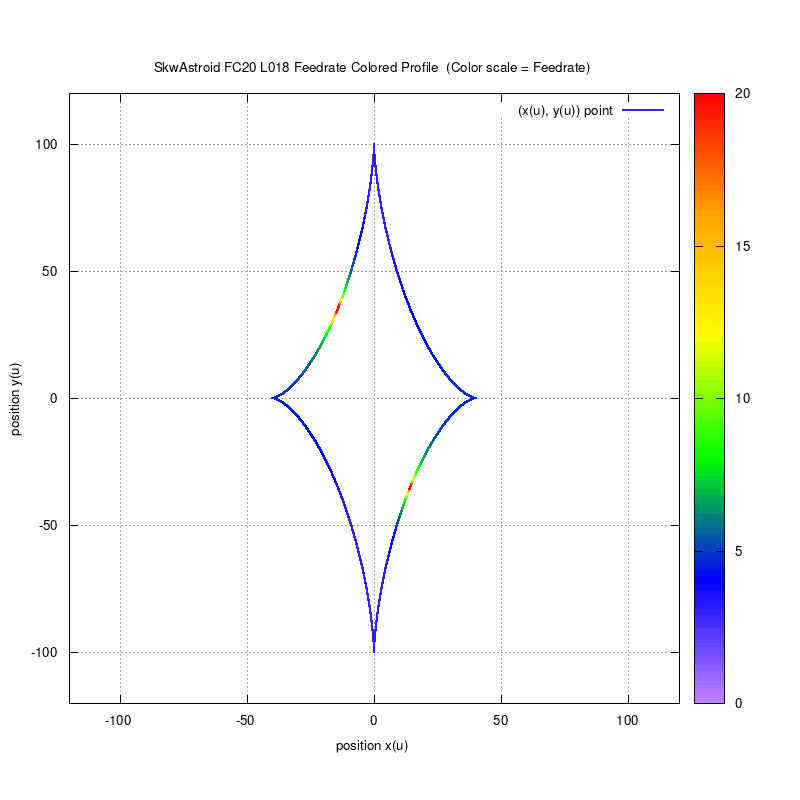
\includegraphics[width=0.75\textwidth]{Chap4/appendix/app-SkwAstroid/plots/18-img-SkwAstroid-FC20-Colored-Feedrate-Profile-data_ngcode.png}
\end{figure}

%% ==================================================
\clearpage
\pagebreak

\begin{figure}
	\caption     {SkwAstroid FC30 Colored Feedrate Profile data ngcode}
	\label{19-img-SkwAstroid-FC30-Colored-Feedrate-Profile-data_ngcode.png}
	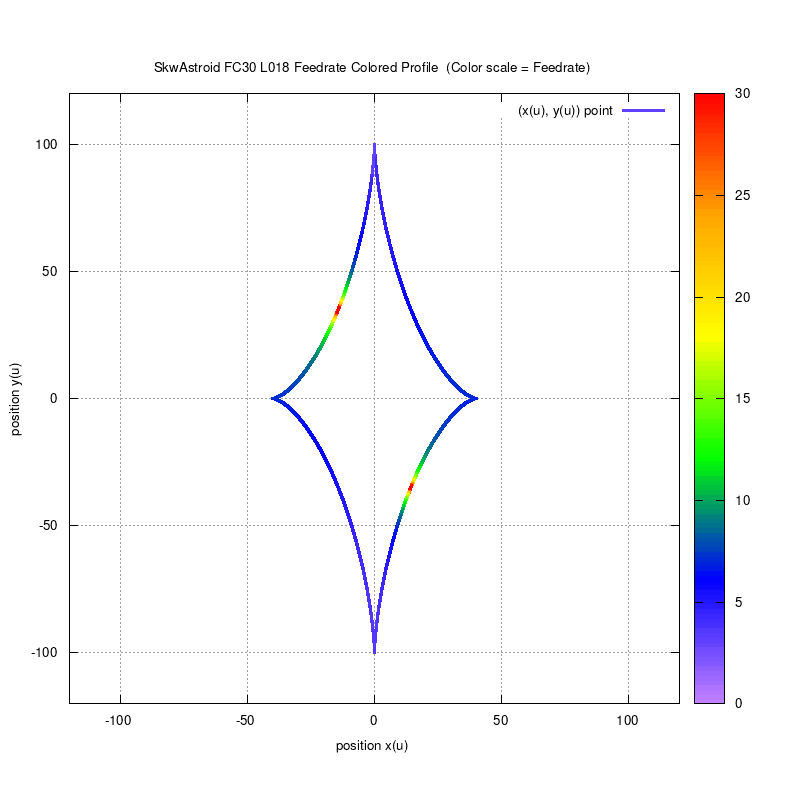
\includegraphics[width=0.75\textwidth]{Chap4/appendix/app-SkwAstroid/plots/19-img-SkwAstroid-FC30-Colored-Feedrate-Profile-data_ngcode.png}
\end{figure}


\begin{figure}
	\caption     {SkwAstroid FC40 Colored Feedrate Profile data ngcode}
	\label{20-img-SkwAstroid-FC40-Colored-Feedrate-Profile-data_ngcode.png}
	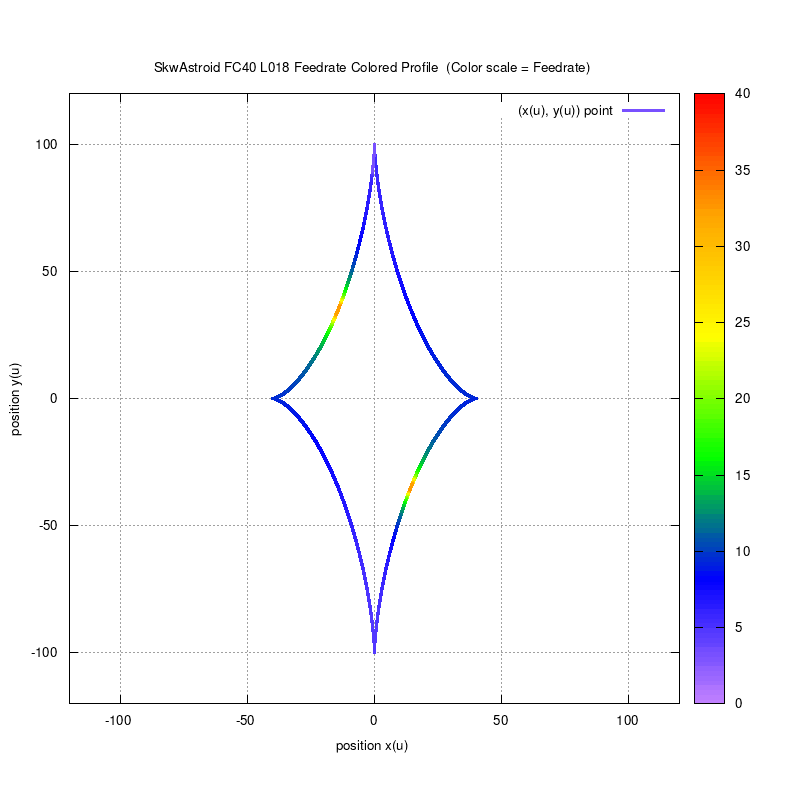
\includegraphics[width=0.75\textwidth]{Chap4/appendix/app-SkwAstroid/plots/20-img-SkwAstroid-FC40-Colored-Feedrate-Profile-data_ngcode.png}
\end{figure}

%% ==================================================
\clearpage
\pagebreak

\begin{figure}
	\caption     {SkwAstroid FC10 Tangential Acceleration}
	\label{21-img-SkwAstroid-FC10-Tangential-Acceleration.pdf}
	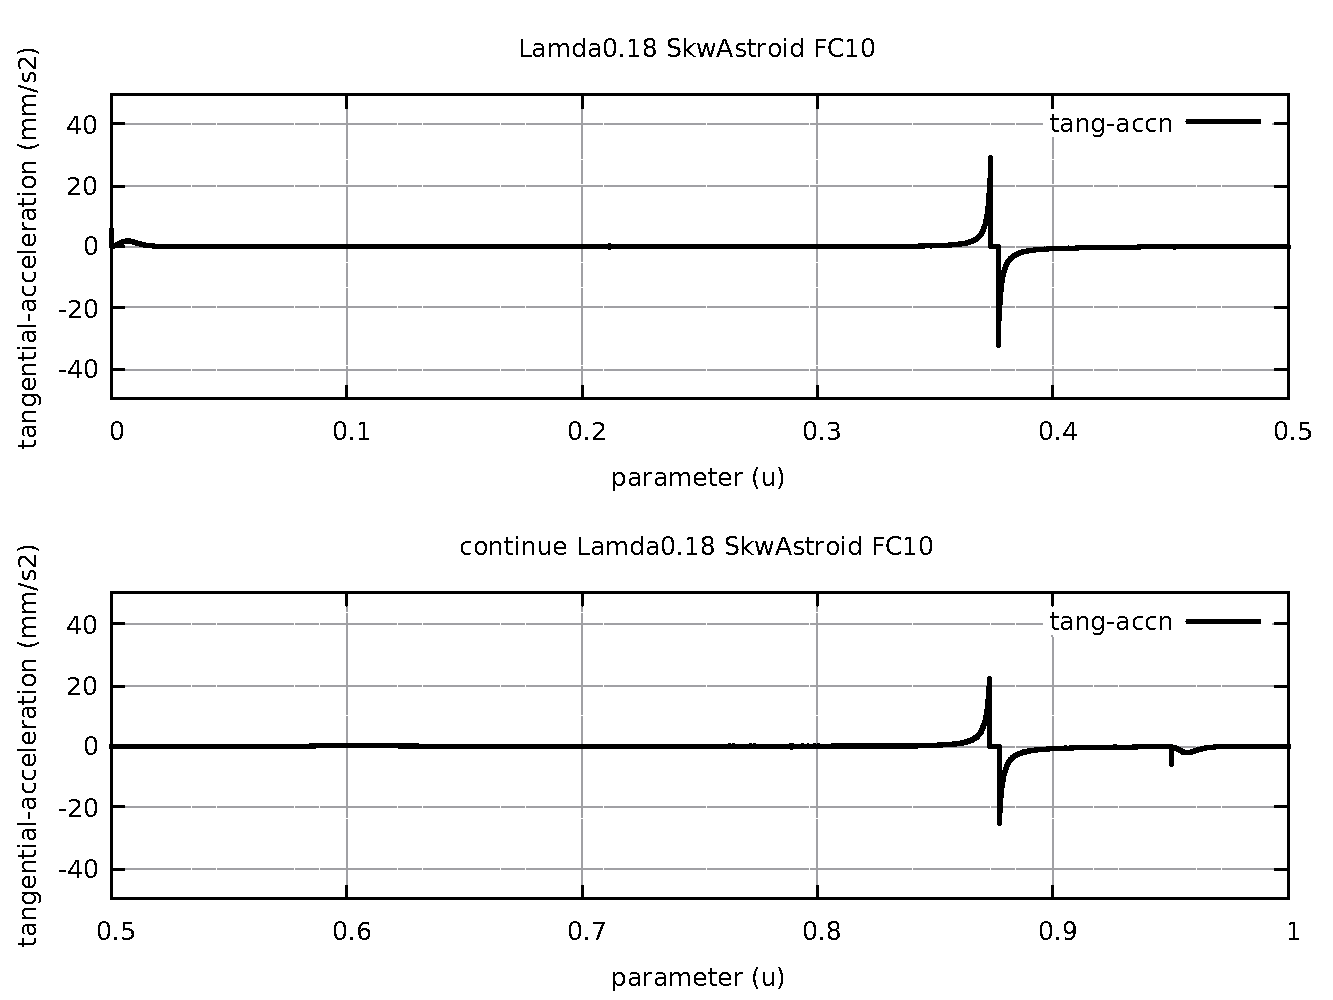
\includegraphics[width=1.00\textwidth]{Chap4/appendix/app-SkwAstroid/plots/21-img-SkwAstroid-FC10-Tangential-Acceleration.pdf}
\end{figure}


\begin{figure}
	\caption     {SkwAstroid FC20 Tangential Acceleration}
	\label{22-img-SkwAstroid-FC20-Tangential-Acceleration.pdf}
	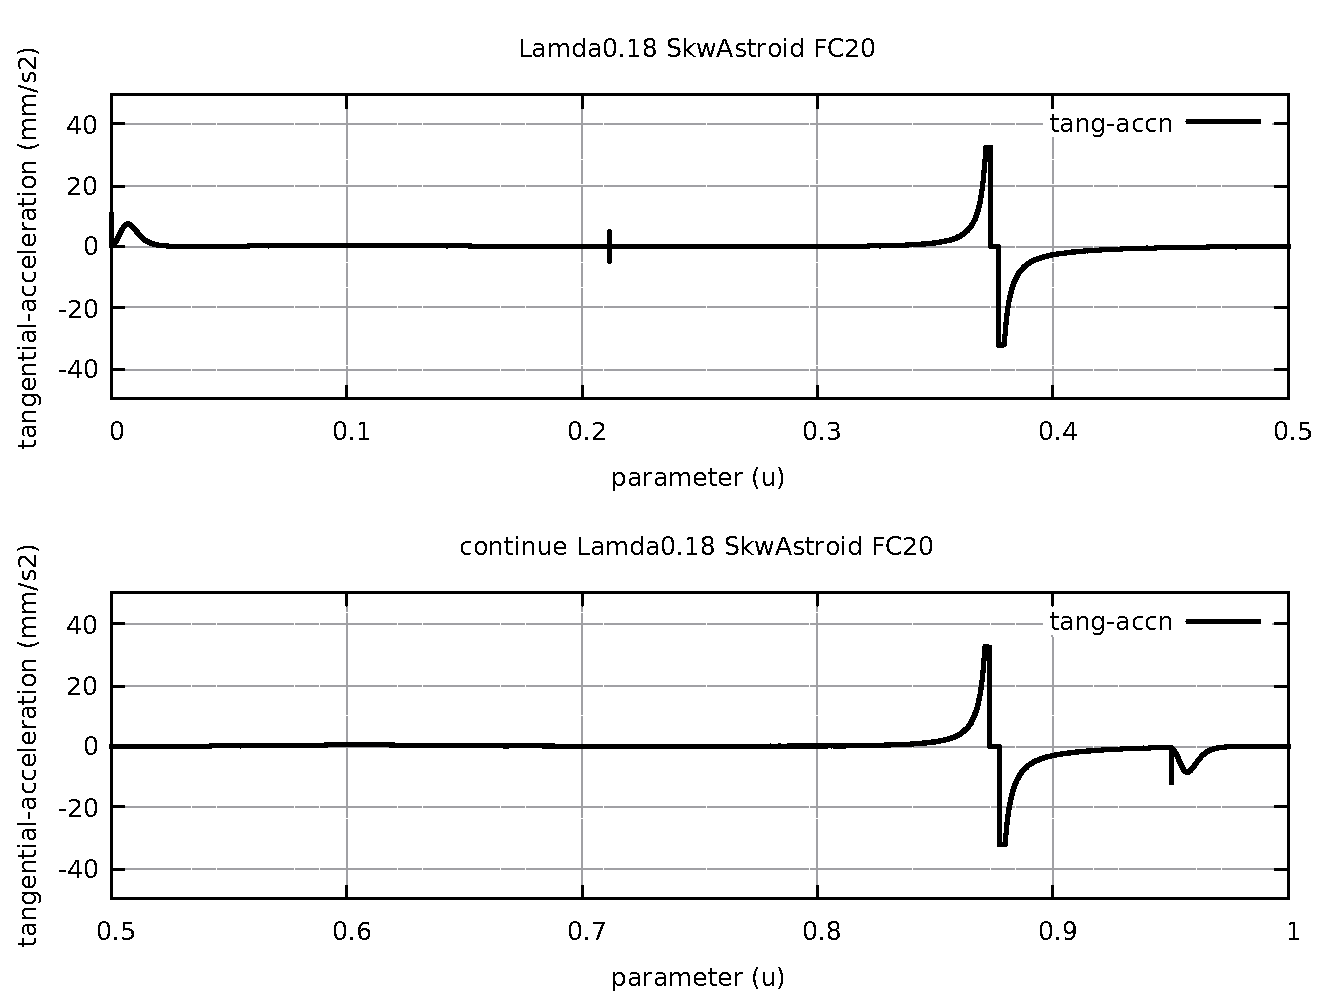
\includegraphics[width=1.00\textwidth]{Chap4/appendix/app-SkwAstroid/plots/22-img-SkwAstroid-FC20-Tangential-Acceleration.pdf}
\end{figure}

%% ==================================================
\clearpage
\pagebreak

\begin{figure}
	\caption     {SkwAstroid FC30 Tangential Acceleration}
	\label{23-img-SkwAstroid-FC30-Tangential-Acceleration.pdf}
	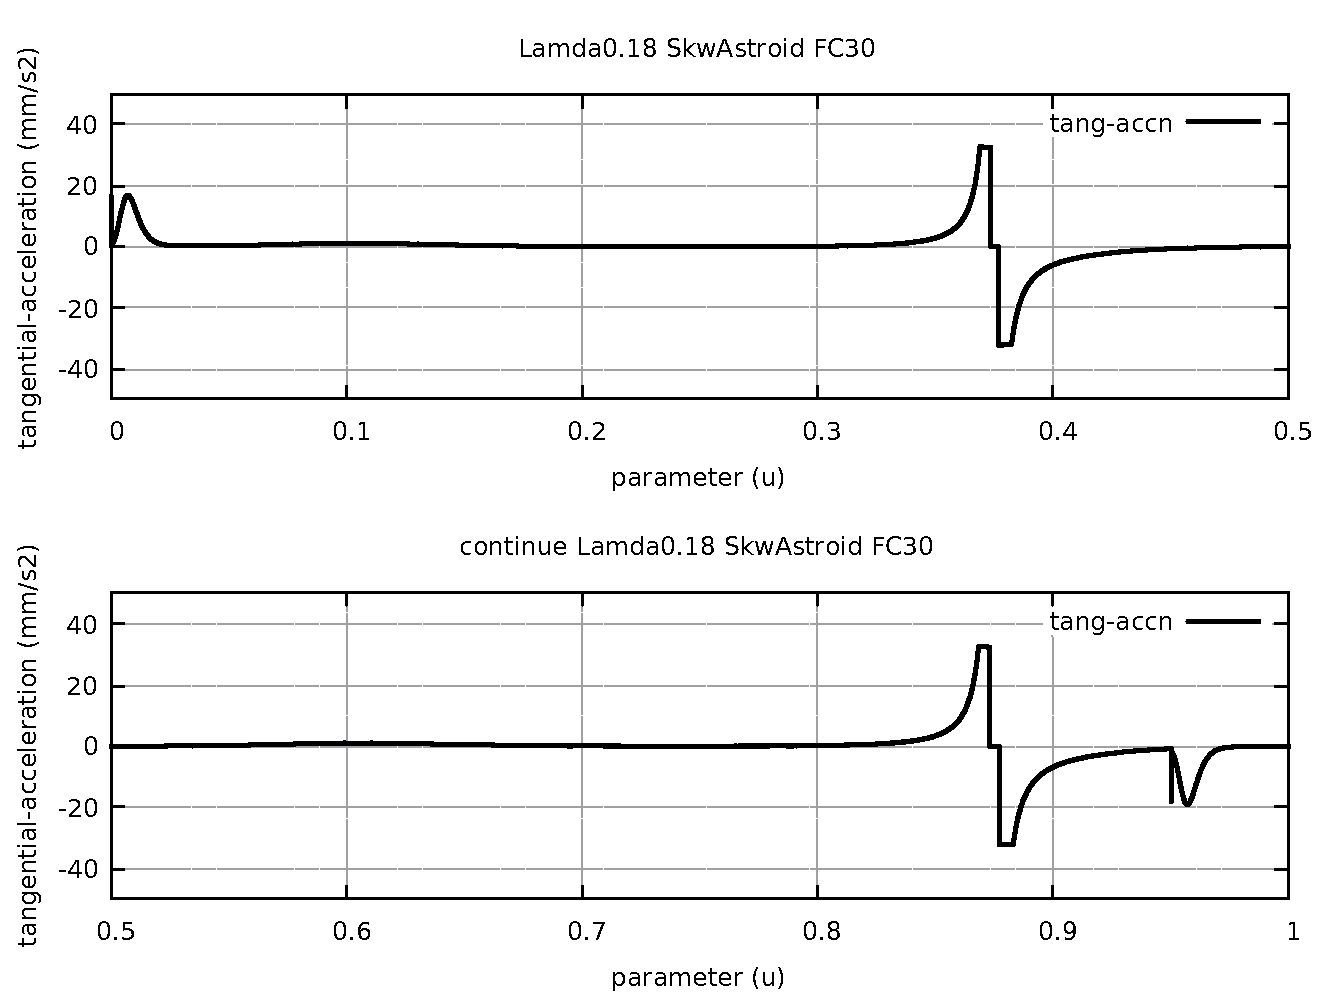
\includegraphics[width=1.00\textwidth]{Chap4/appendix/app-SkwAstroid/plots/23-img-SkwAstroid-FC30-Tangential-Acceleration.pdf}
\end{figure}


\begin{figure}
	\caption     {SkwAstroid FC40 Tangential Acceleration}
	\label{24-img-SkwAstroid-FC40-Tangential-Acceleration.pdf}
	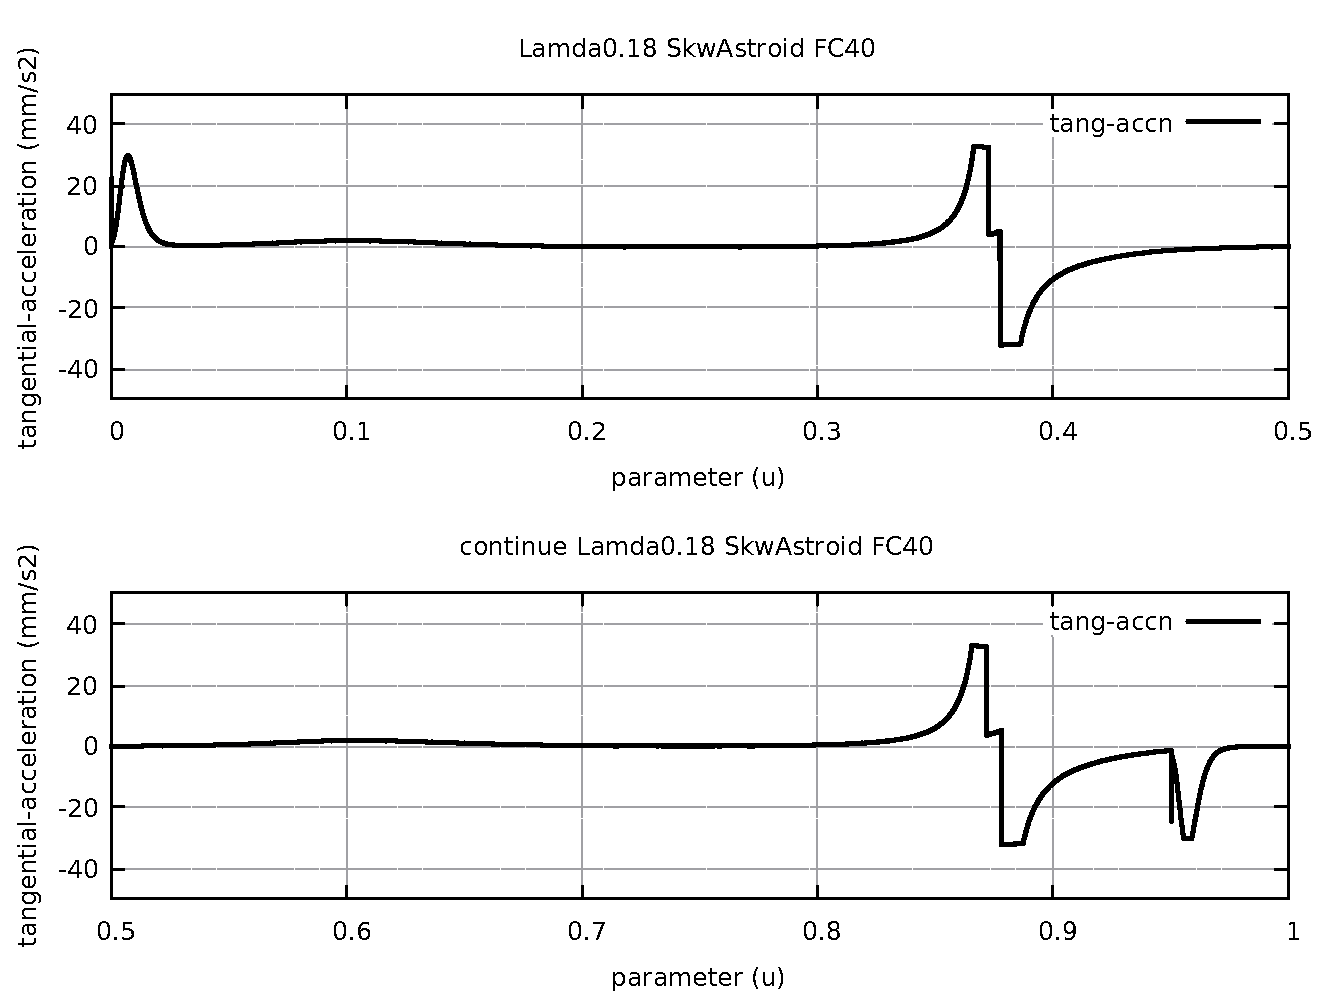
\includegraphics[width=1.00\textwidth]{Chap4/appendix/app-SkwAstroid/plots/24-img-SkwAstroid-FC40-Tangential-Acceleration.pdf}
\end{figure}

%% ==================================================
\clearpage
\pagebreak

\begin{figure}
	\caption     {SkwAstroid FC20 Nominal Separation NAL and NCL}
	\label{25-img-SkwAstroid-FC20-Nominal-Separation-NAL-and-NCL.pdf}
	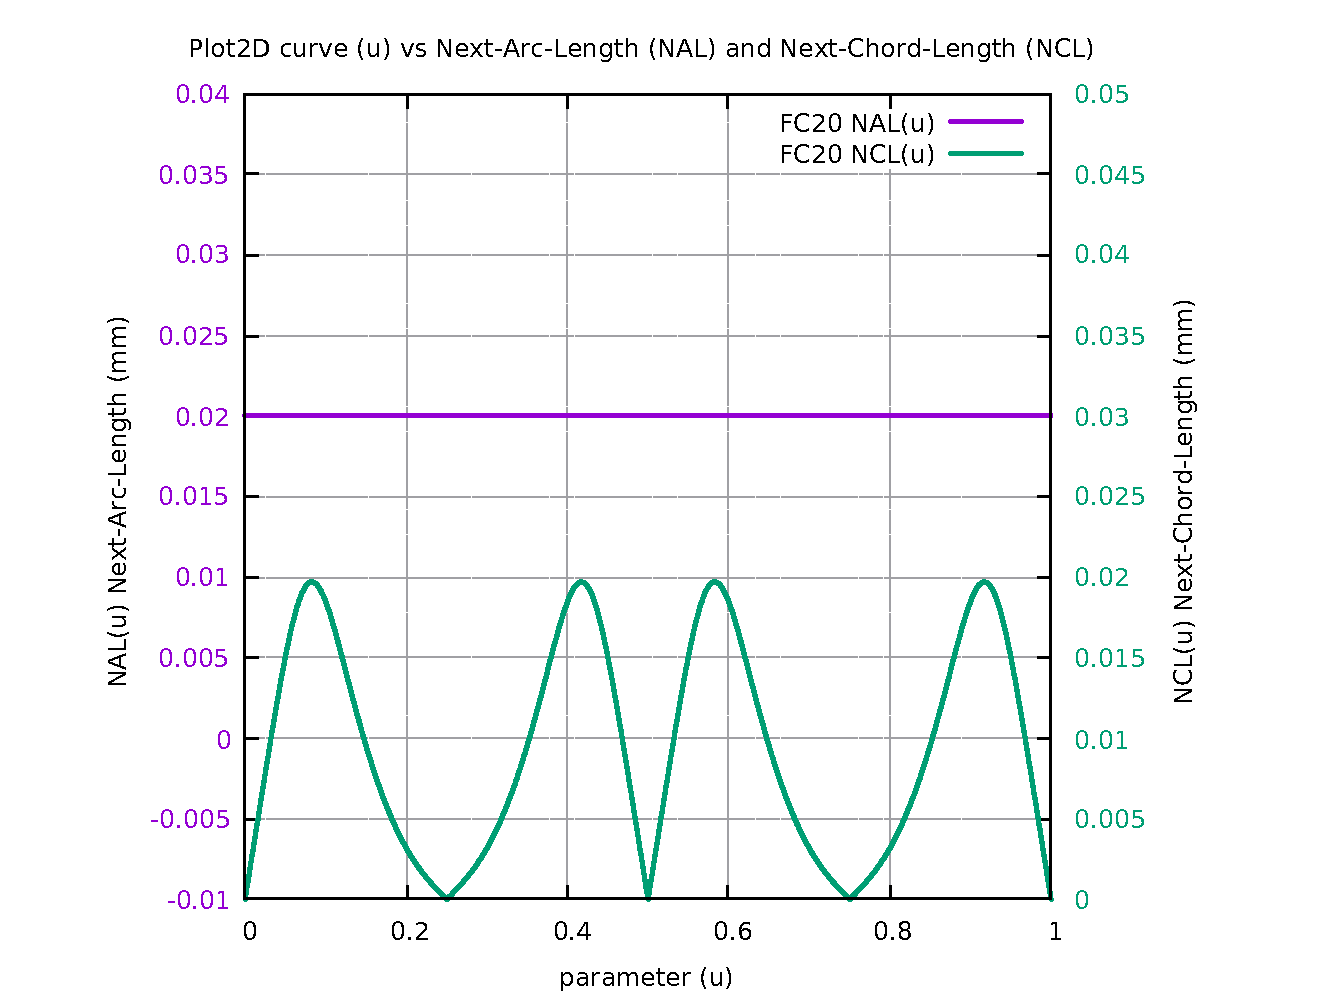
\includegraphics[width=1.00\textwidth]{Chap4/appendix/app-SkwAstroid/plots/25-img-SkwAstroid-FC20-Nominal-Separation-NAL-and-NCL.pdf}
\end{figure}


\begin{figure}
	\caption     {SkwAstroid Difference SAL minus SCL for FC10 FC20 FC30 FC40}
	\label{26-img-SkwAstroid-Difference-SAL-minus-SCL-for-FC10-FC20-FC30-FC40.pdf}
	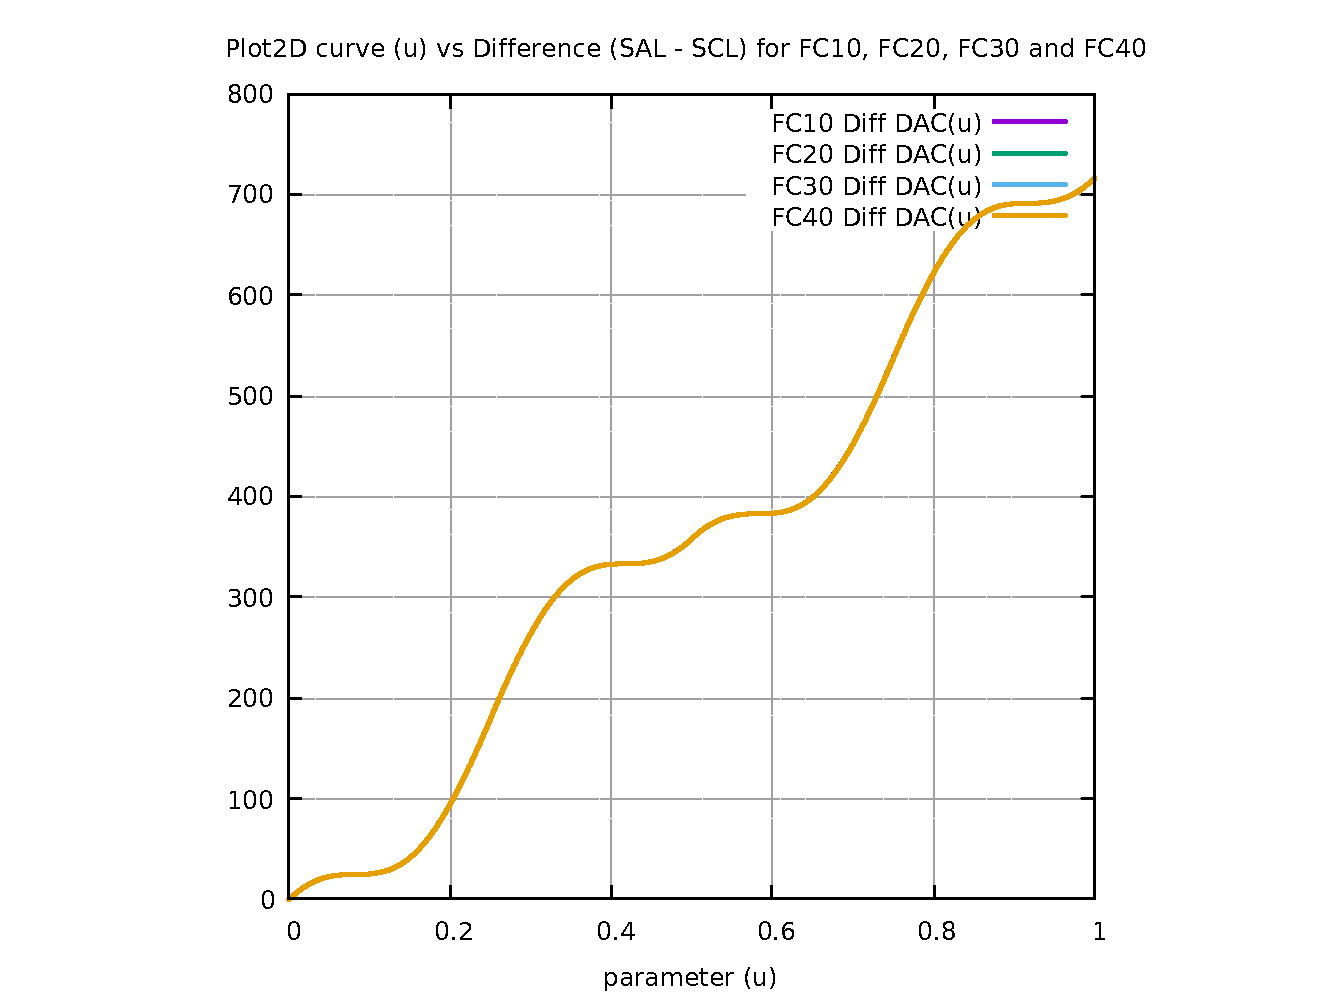
\includegraphics[width=1.00\textwidth]{Chap4/appendix/app-SkwAstroid/plots/26-img-SkwAstroid-Difference-SAL-minus-SCL-for-FC10-FC20-FC30-FC40.pdf}
\end{figure}


%% ==================================================
\clearpage
\pagebreak

\begin{figure}
	\caption     {SkwAstroid FC10 FrateCmd CurrFrate X-Frate Y-Frate}
	\label{27-img-SkwAstroid-FC10-FrateCmd-CurrFrate-X-Frate-Y-Frate.pdf}
	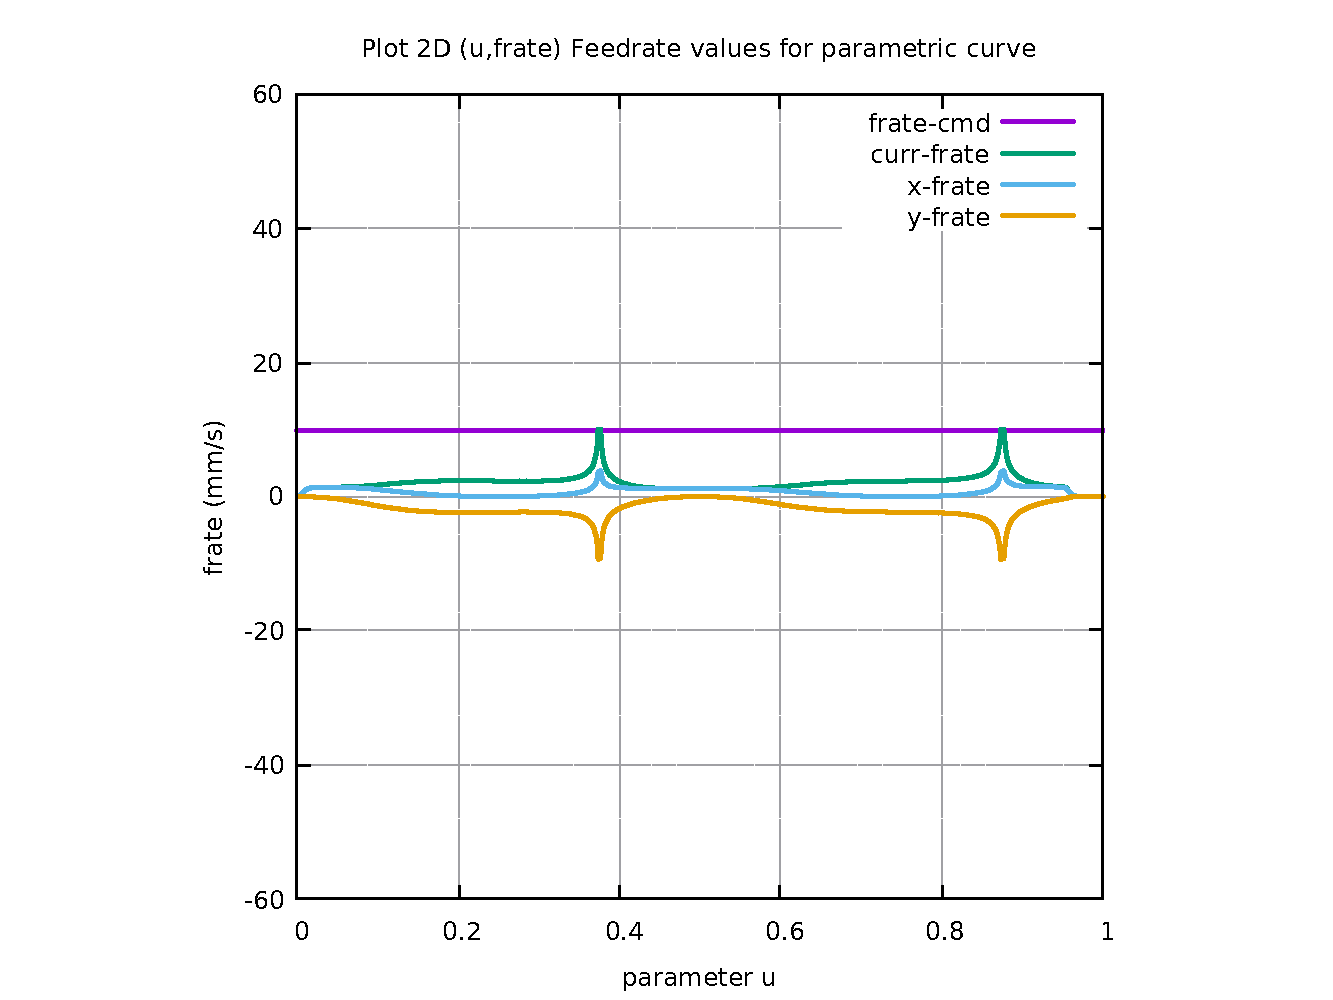
\includegraphics[width=1.00\textwidth]{Chap4/appendix/app-SkwAstroid/plots/27-img-SkwAstroid-FC10-FrateCmd-CurrFrate-X-Frate-Y-Frate.pdf}
\end{figure}


\begin{figure}
	\caption     {SkwAstroid FC20 FrateCmd CurrFrate X-Frate Y-Frate}
	\label{28-img-SkwAstroid-FC20-FrateCmd-CurrFrate-X-Frate-Y-Frate.pdf}
	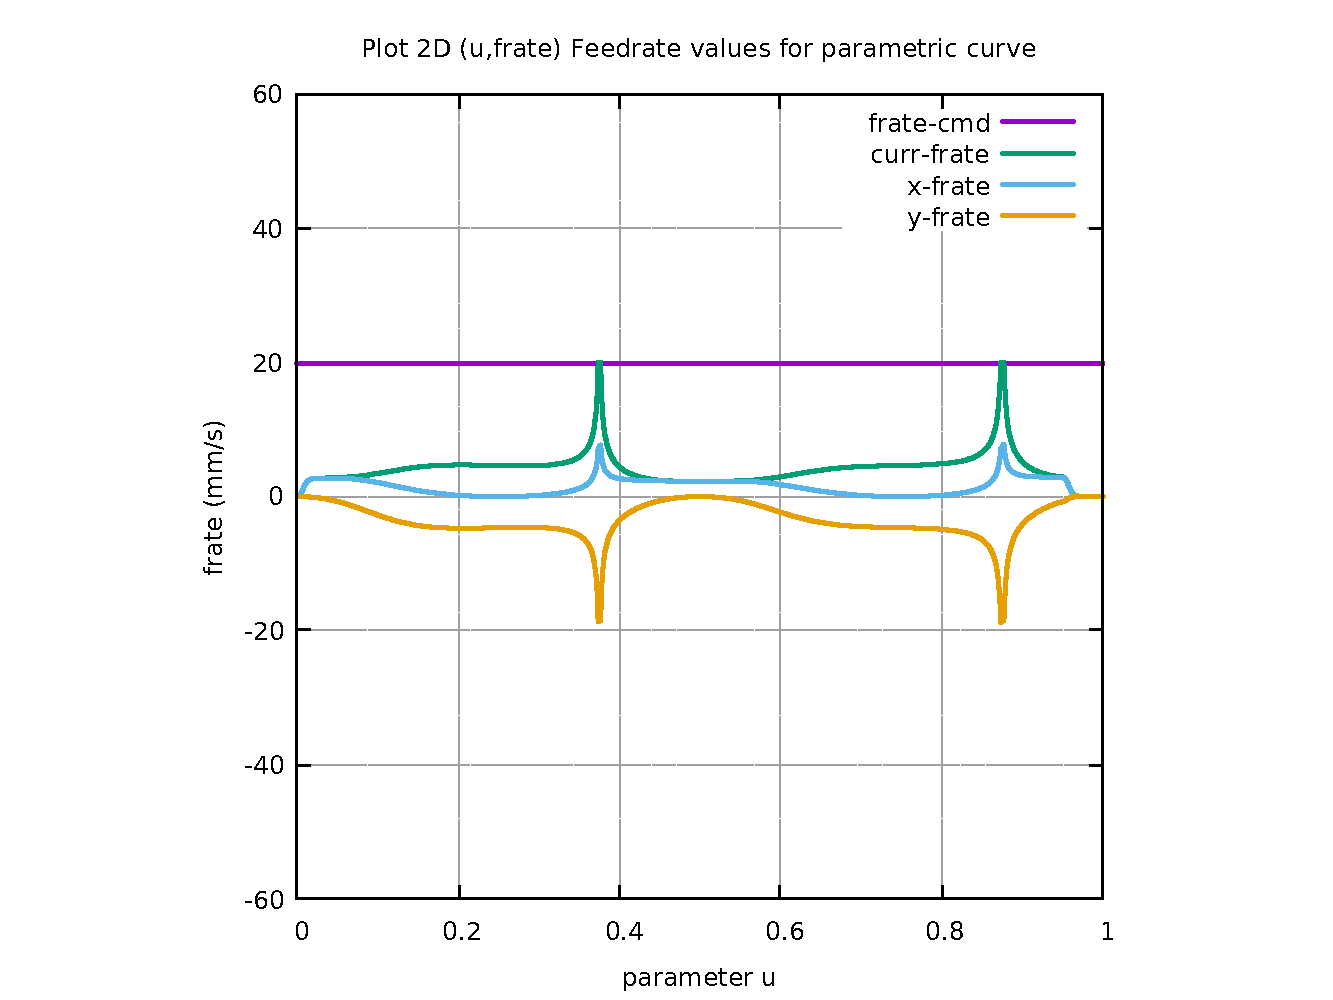
\includegraphics[width=1.00\textwidth]{Chap4/appendix/app-SkwAstroid/plots/28-img-SkwAstroid-FC20-FrateCmd-CurrFrate-X-Frate-Y-Frate.pdf}
\end{figure}


%% ==================================================
\clearpage
\pagebreak

\begin{figure}
	\caption     {SkwAstroid FC30 FrateCmd CurrFrate X-Frate Y-Frate}
	\label{29-img-SkwAstroid-FC30-FrateCmd-CurrFrate-X-Frate-Y-Frate.pdf}
	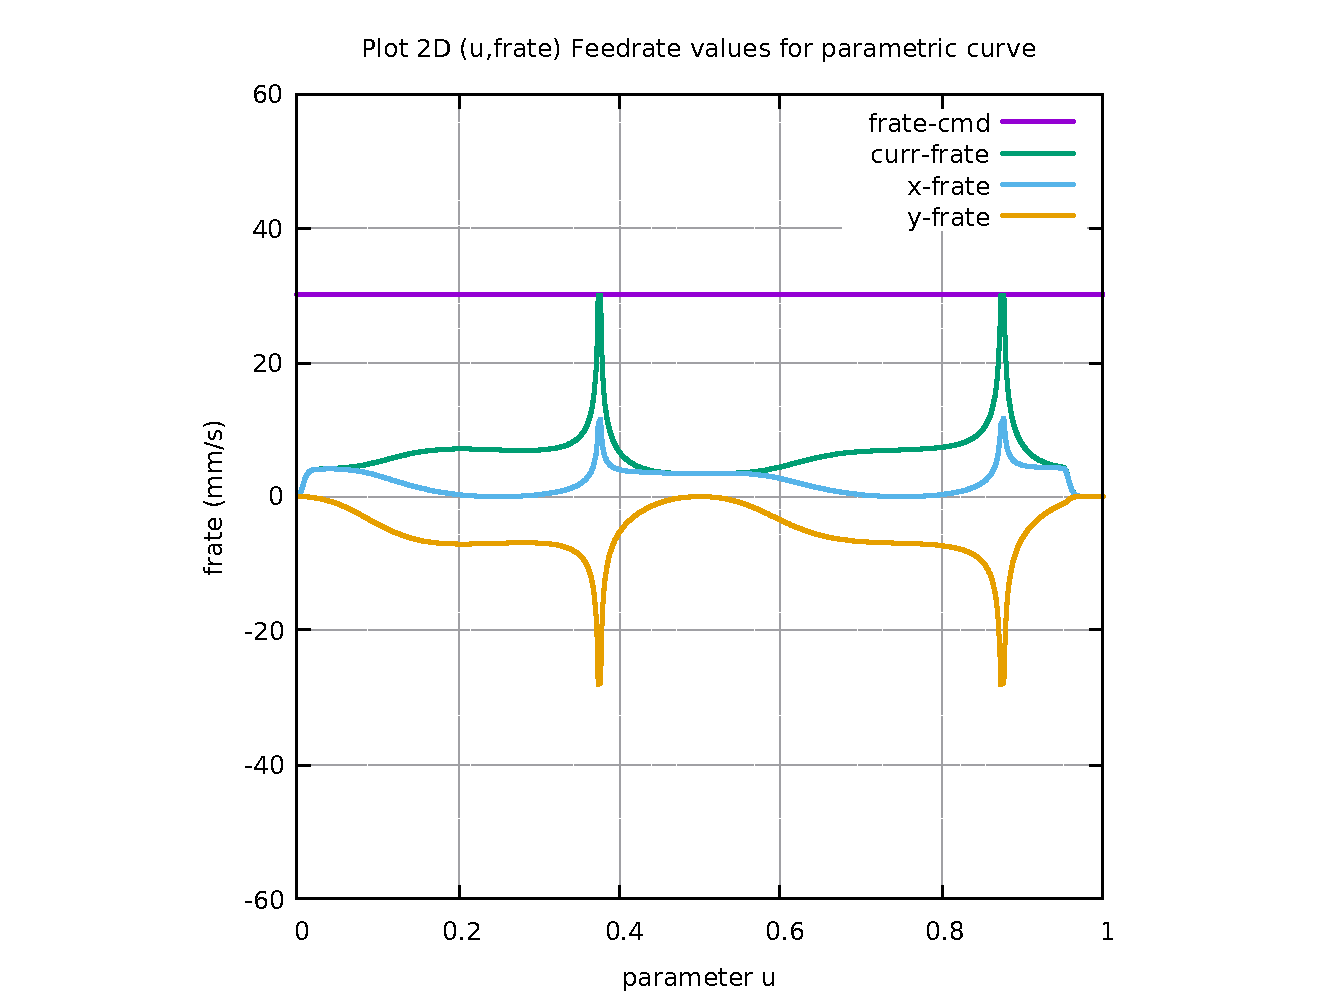
\includegraphics[width=1.00\textwidth]{Chap4/appendix/app-SkwAstroid/plots/29-img-SkwAstroid-FC30-FrateCmd-CurrFrate-X-Frate-Y-Frate.pdf}
\end{figure}


\begin{figure}
	\caption     {SkwAstroid FC40 FrateCmd CurrFrate X-Frate Y-Frate}
	\label{30-img-SkwAstroid-FC40-FrateCmd-CurrFrate-X-Frate-Y-Frate.pdf}
	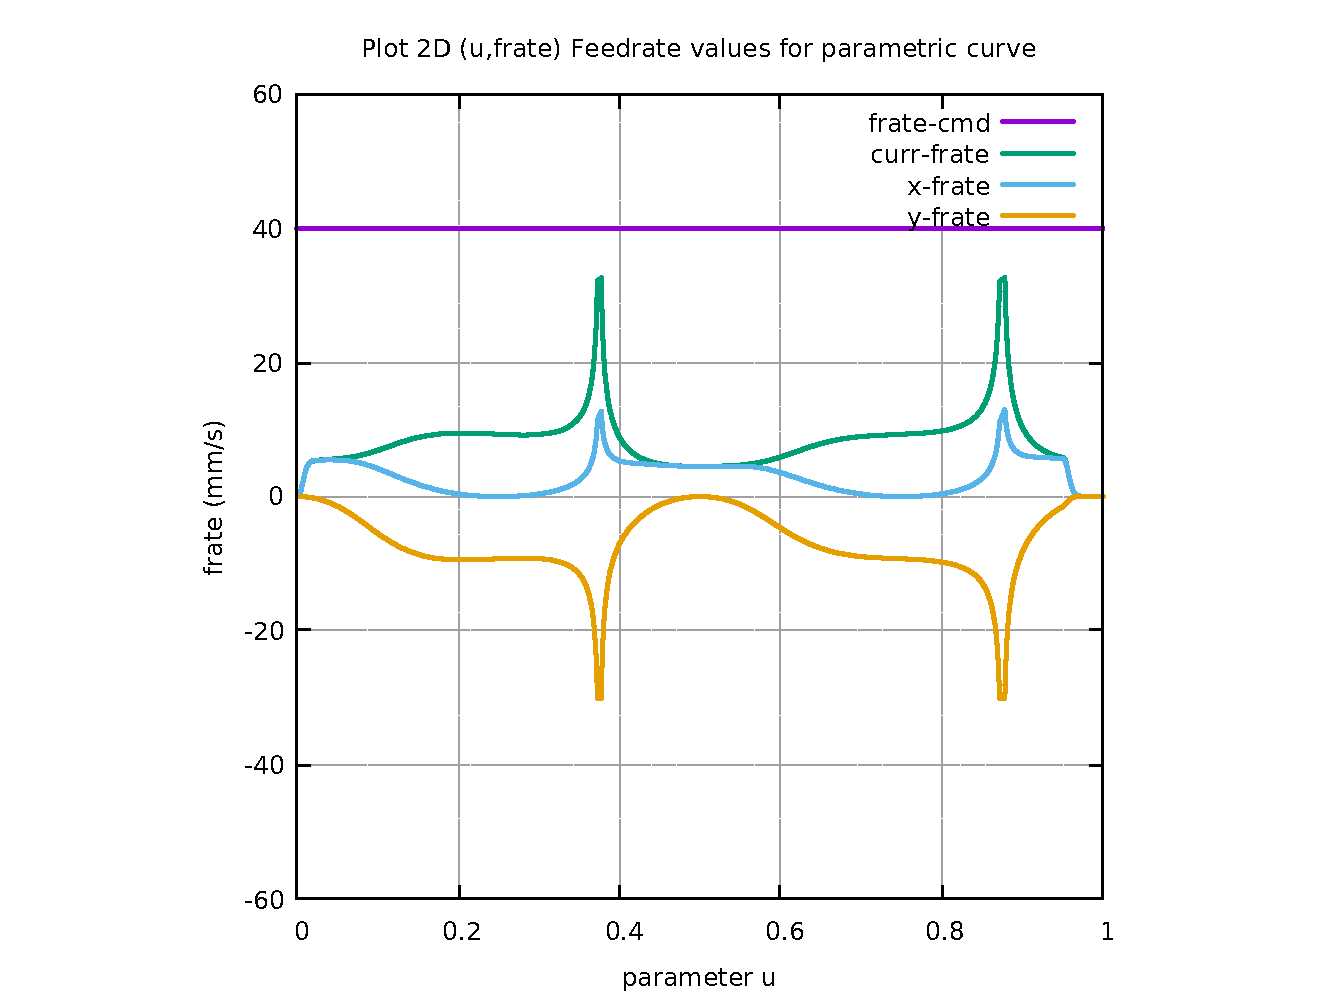
\includegraphics[width=1.00\textwidth]{Chap4/appendix/app-SkwAstroid/plots/30-img-SkwAstroid-FC40-FrateCmd-CurrFrate-X-Frate-Y-Frate.pdf}
\end{figure}


%% ==================================================
\clearpage
\pagebreak

\begin{figure}
	\caption     {SkwAstroid FC10 Four Components FeedrateLimit}
	\label{31-img-SkwAstroid-FC10-Four-Components-FeedrateLimit.pdf}
	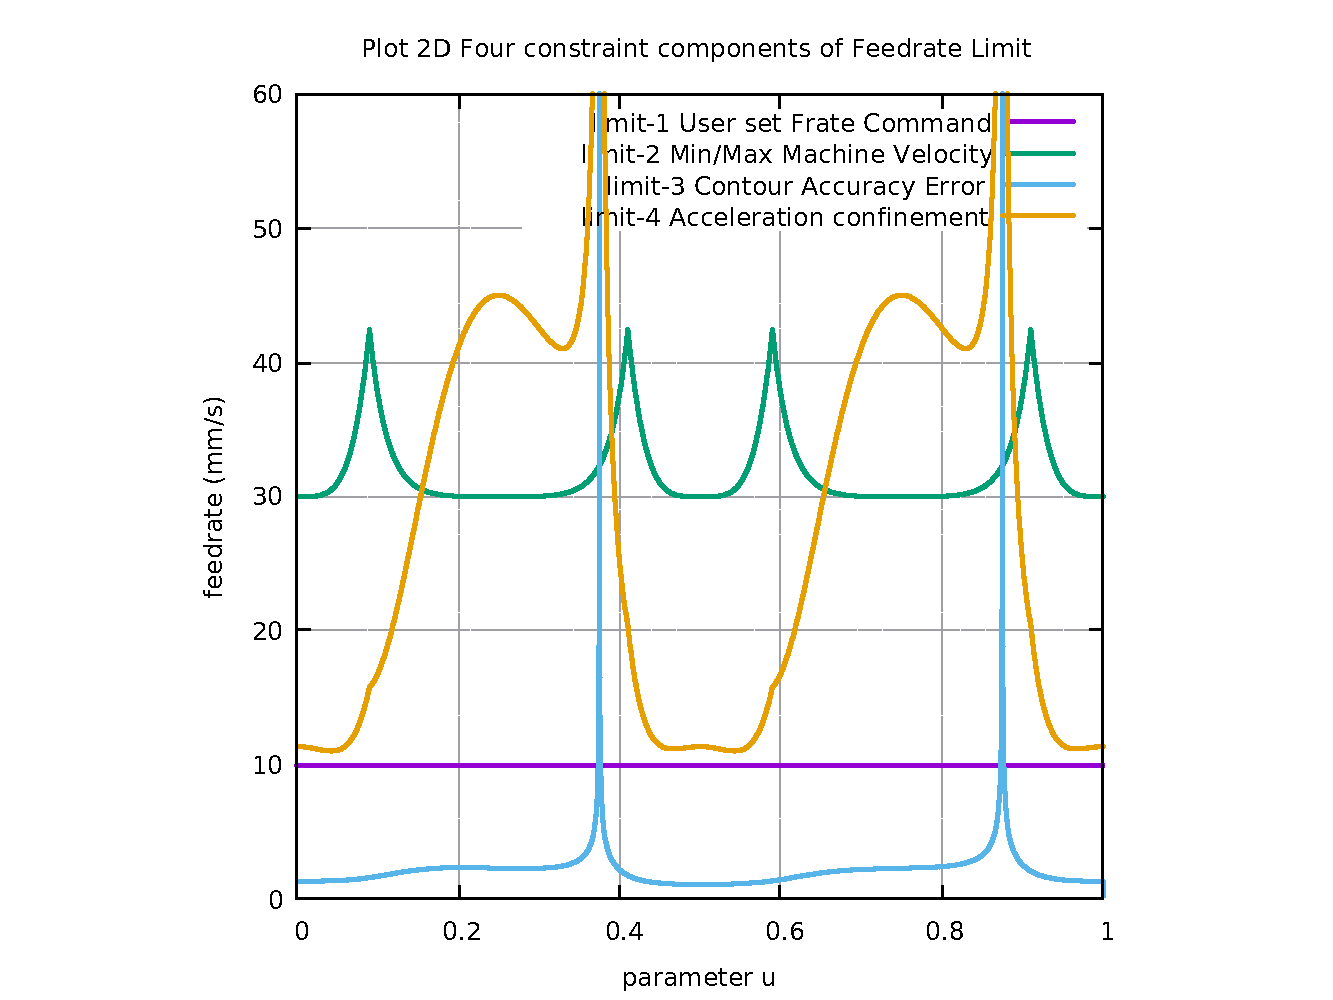
\includegraphics[width=1.00\textwidth]{Chap4/appendix/app-SkwAstroid/plots/31-img-SkwAstroid-FC10-Four-Components-FeedrateLimit.pdf}
\end{figure}


\begin{figure}
	\caption     {SkwAstroid FC20 Four Components FeedrateLimit}
	\label{32-img-SkwAstroid-FC20-Four-Components-FeedrateLimit.pdf}
	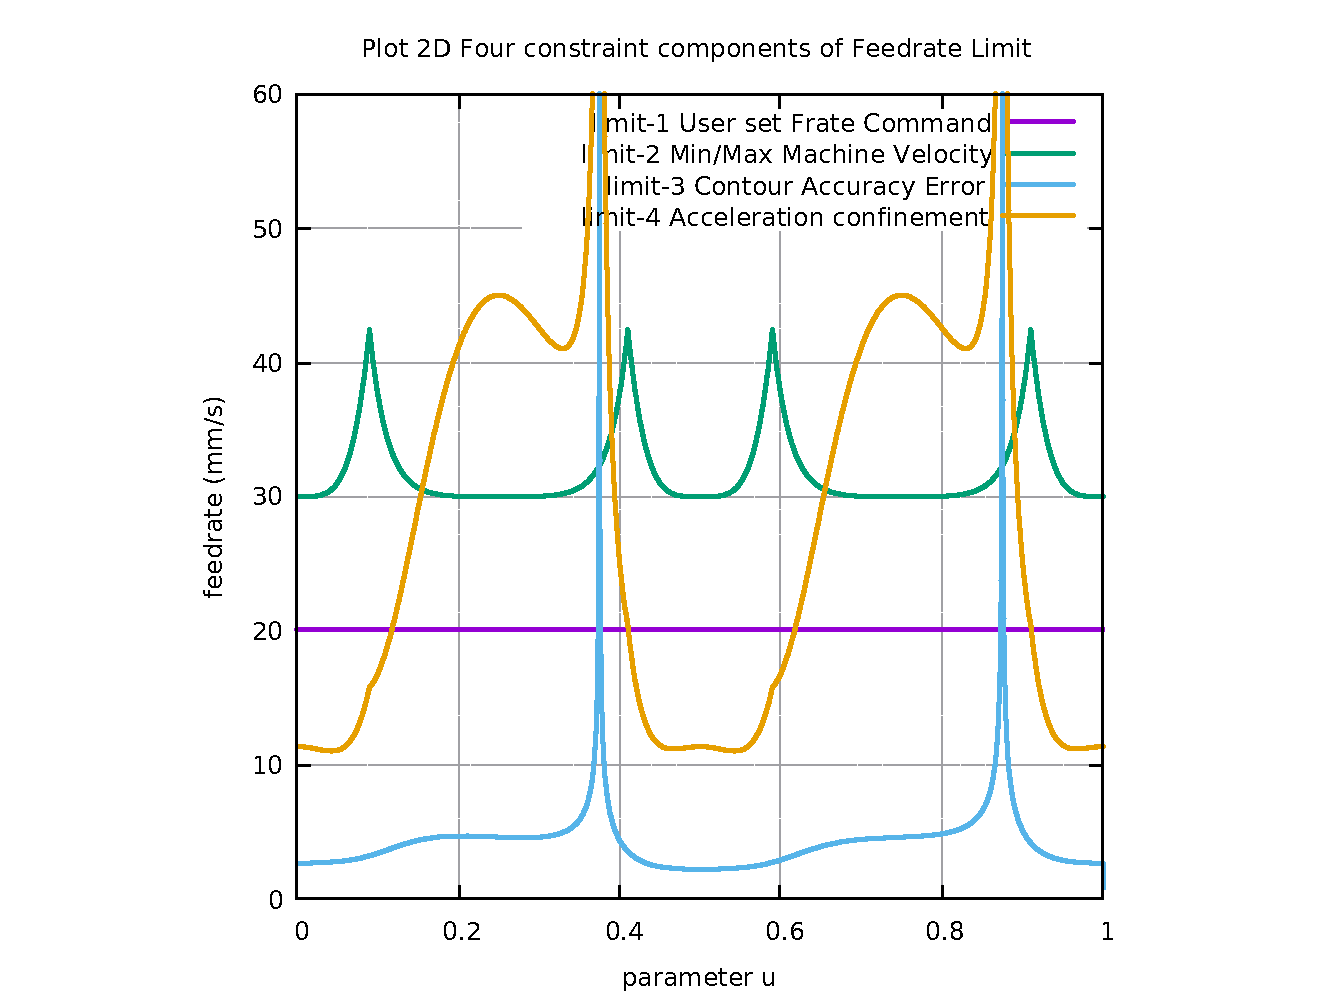
\includegraphics[width=1.00\textwidth]{Chap4/appendix/app-SkwAstroid/plots/32-img-SkwAstroid-FC20-Four-Components-FeedrateLimit.pdf}
\end{figure}


%% ==================================================
\clearpage
\pagebreak

\begin{figure}
	\caption     {SkwAstroid FC30 Four Components FeedrateLimit}
	\label{33-img-SkwAstroid-FC30-Four-Components-FeedrateLimit.pdf}
	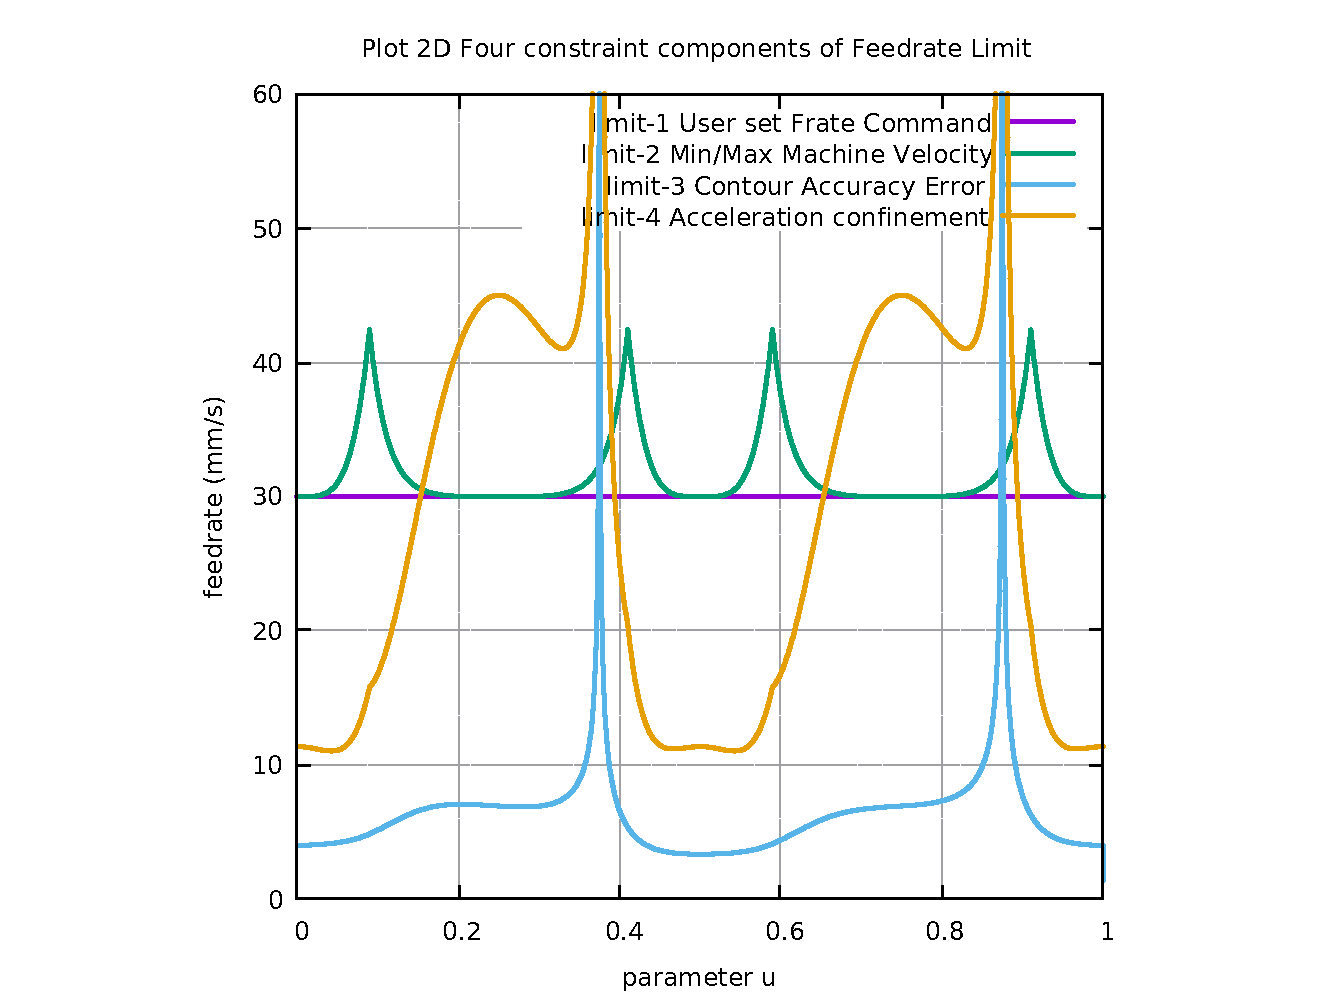
\includegraphics[width=1.00\textwidth]{Chap4/appendix/app-SkwAstroid/plots/33-img-SkwAstroid-FC30-Four-Components-FeedrateLimit.pdf}
\end{figure}


\begin{figure}
	\caption     {SkwAstroid FC40 Four Components FeedrateLimit}
	\label{34-img-SkwAstroid-FC40-Four-Components-FeedrateLimit.pdf}
	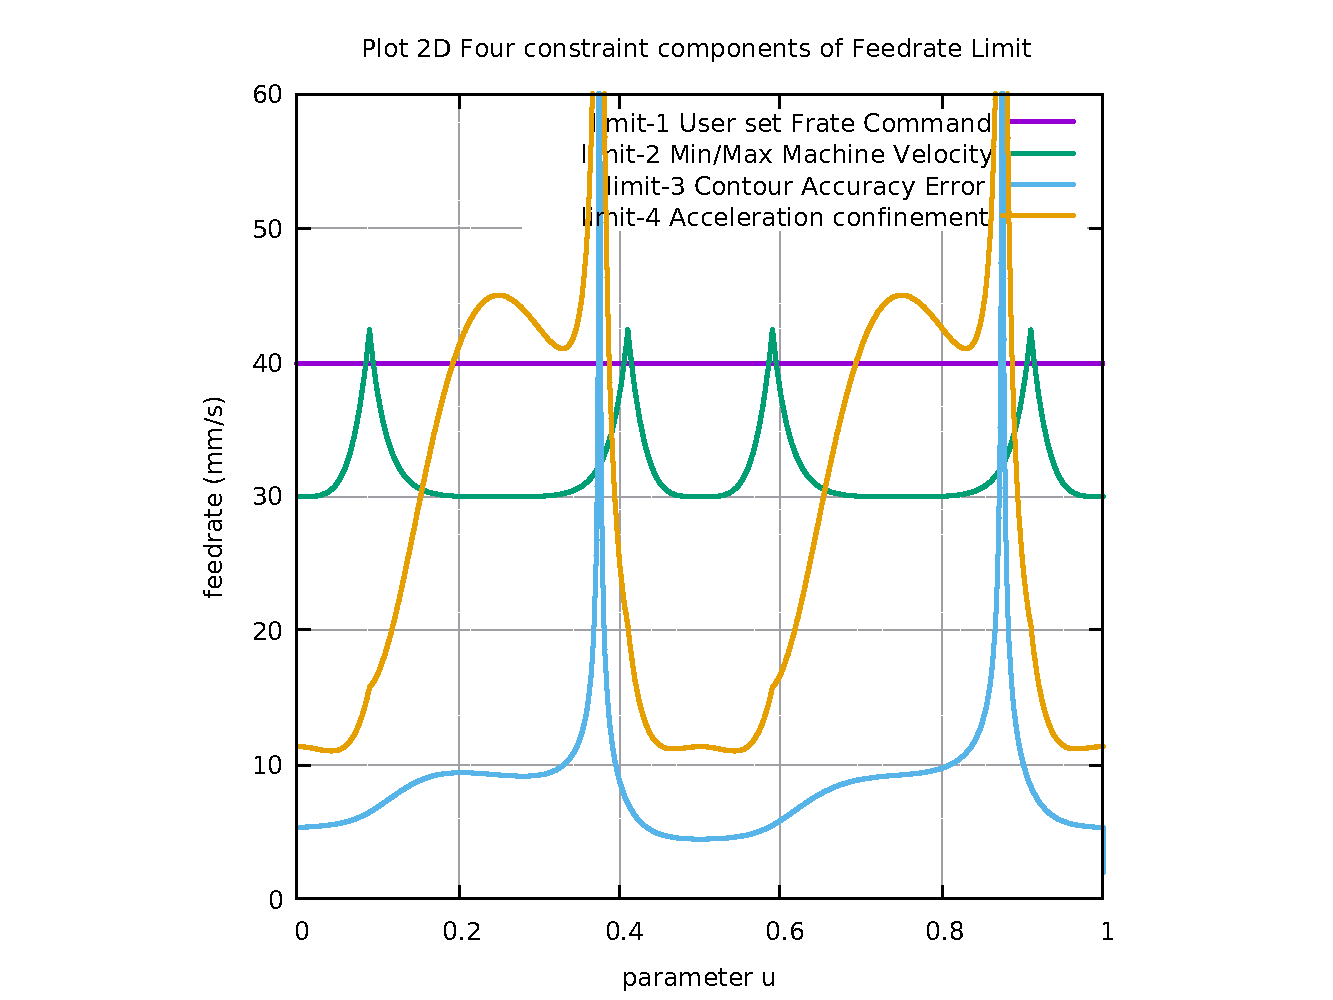
\includegraphics[width=1.00\textwidth]{Chap4/appendix/app-SkwAstroid/plots/34-img-SkwAstroid-FC40-Four-Components-FeedrateLimit.pdf}
\end{figure}


%% =======================================
\clearpage
\pagebreak

\begin{figure}
	\centering
	\caption     {SkwAstroid Histogram Points FC10 FC20 FC30 FC40}
	\label{35-img-SkwAstroid-Histogram-Points-FC10-FC20-FC30-FC40.pdf}
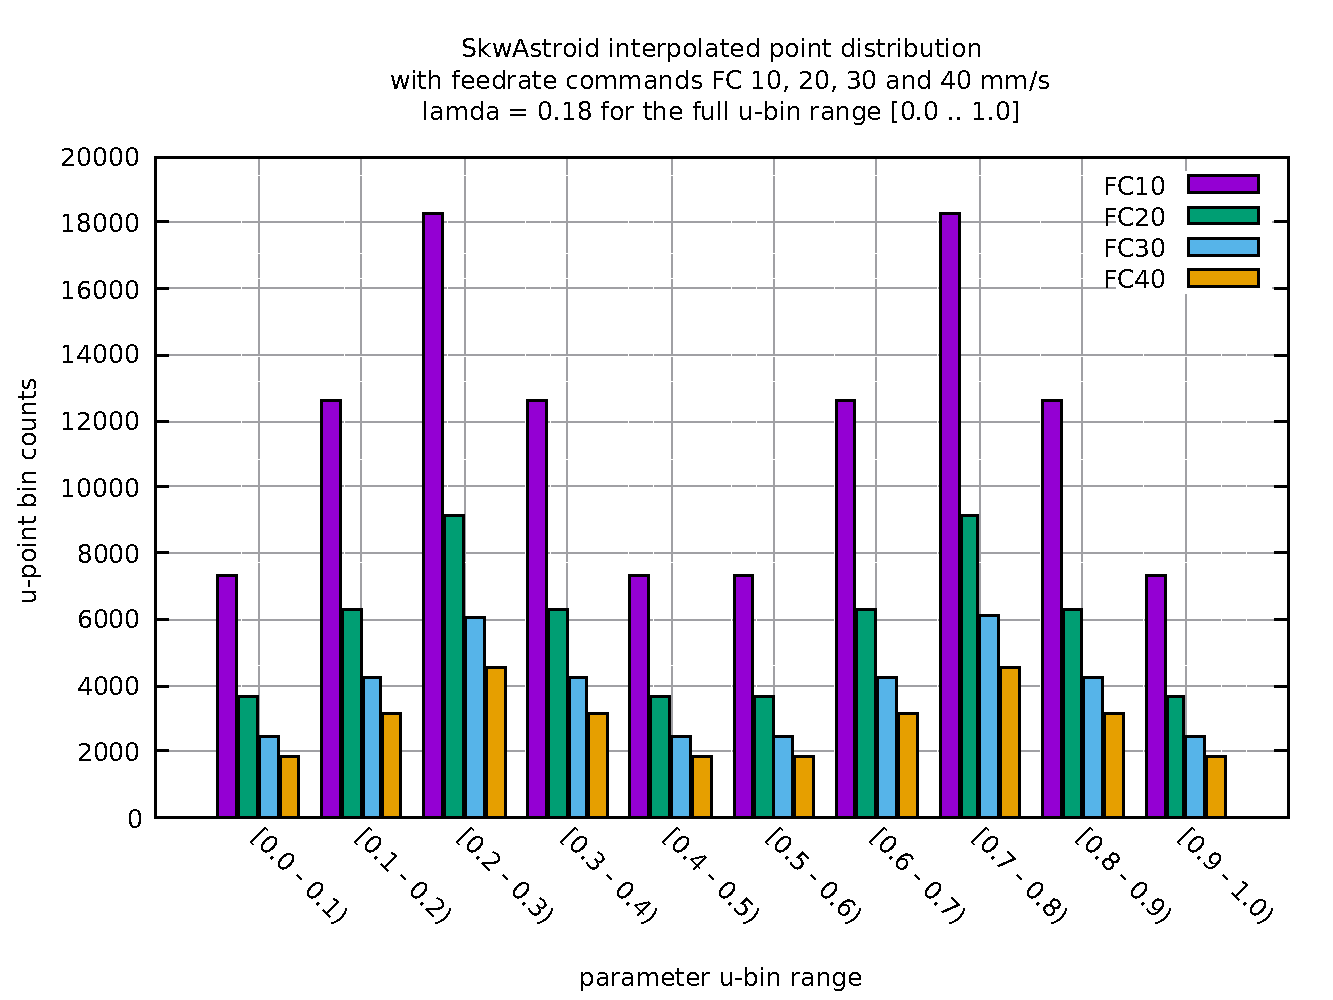
\includegraphics[width=1.00\textwidth]{Chap4/appendix/app-SkwAstroid/plots/35-img-SkwAstroid-Histogram-Points-FC10-FC20-FC30-FC40.pdf} 
\end{figure}


\begin{table}[ht]
%% \begin{center}
\caption    {SkwAstroid Table distribution of interpolated points}
\label  {tab-SkwAstroid Table distribution of interpolated points}
	
%% IMPORTANT TO SCALEBOX BELOW
\scalebox{0.80}{
		
%% START COPY AND PASTE BELOW HERE
%% FROM \begin{tabular} UNTIL \end{tabular)
%% Note: adjust last p{} to get line width correct
		
\begin{tabular}{ p{4.5cm} p{1.5cm} p{1.5cm} p{1.5cm} p{7.50cm} }
\hline
	&		&		&		&		\\
BINS	&	FC10	&	FC20	&	FC30	&	FC40	\\
&		&		&		&		\\
0.0 - 0.1	&	7322	&	3661	&	2441	&	1831	\\
0.1 - 0.2	&	12603	&	6302	&	4202	&	3151	\\
0.2 - 0.3	&	18245	&	9123	&	6081	&	4562	\\
0.3 - 0.4	&	12604	&	6302	&	4202	&	3151	\\
0.4 - 0.5	&	7322	&	3662	&	2442	&	1832	\\
0.5 - 0.6	&	7323	&	3662	&	2442	&	1832	\\
0.6 - 0.7	&	12603	&	6302	&	4201	&	3151	\\
0.7 - 0.8	&	18244	&	9122	&	6082	&	4561	\\
0.8 - 0.9	&	12604	&	6303	&	4202	&	3152	\\
0.9 - 1.0	&	7324	&	3663	&	2443	&	1833	\\
&		&		&		&		\\
Tot Counts	&	116194	&	58102	&	38738	&	29056	\\
&		&		&		&		\\
\hline	
\end{tabular}
		
%% END COPY AND PASTE ABOVE HERE
		
}   %% IMPORTANT FOR SCALEBOX CLOSING
	
\end{table}
%% \end{landscape}

%% SkwAstroid SUMMARY TABLE
%% ========================================================
\clearpage
\pagebreak
\begin{landscape}
	
\begin{table}[ht]
%% \begin{center}
\caption       {SkwAstroid Table FC10-20-30-40 Run Performance data}
\label{tab-app4-SkwAstroid-Table-FC10-20-30-40-Run-Performance-data}
		
%% IMPORTANT TO SCALEBOX BELOW
\scalebox{0.90}{
			
%% START COPY AND PASTE BELOW HERE
%% FROM \begin{tabular} UNTIL \end{tabular)
			
			
\begin{tabular}{ p{0.2cm} p{8.80cm} p{4.00cm} p{4.0cm} p{4.00cm} p{4.0cm}}
	\hline
	&		&		&		&		&		\\
	1	&	Curve Type	&	SKEWED-ASTROID	&	SKEWED-ASTROID	&	SKEWED-ASTROID	&	SKEWED-ASTROID	\\
	2	&	User Feedrate Command FC(mm/s)                   	&	FC10	&	FC20	&	FC30	&	FC40	\\
	3	&	User Lamda Acceleration Safety Factor	&	0.18	&	0.18	&	0.18	&	0.18	\\
	&		&		&		&		&		\\
	4	&	Total Iterpolated Points (TIP)	&	116194	&	58102	&	38738	&	29056	\\
	5	&	Total Sum-Chord-Error (SCE) (mm)	&	5.163683043374E-04	&	1.032591177038E-03	&	1.548668518105E-03	&	2.064600313211E-03	\\
	6	&	Ratio 1 = (SCE/TIP) = Chord-Error/Point	&	4.444056908225E-09	&	1.777234775714E-08	&	3.997905150386E-08	&	7.105834841547E-08	\\
	&		&		&		&		&		\\
	7	&	Total Sum-Arc-Length (SAL) (mm)	&	1.161845691077E+03	&	1.161851349542E+03	&	1.161856975395E+03	&	1.161862568638E+03	\\
	8	&	Total Sum-Chord-Length (SCL) (mm)	&	4.457142858819E+02	&	4.457142855374E+02	&	4.457142846207E+02	&	4.457142831748E+02	\\
	9	&	Difference = (SAL – SCL) (mm)	&	7.161314051951E+02	&	7.161370640044E+02	&	7.161426907744E+02	&	7.161482854628E+02	\\
	10	&	Percentage Difference = (SAL – SCL)/SAL	&	6.163739390653E+01	&	6.163758077028E+01	&	6.163776660469E+01	&	6.163795140613E+01	\\
	&		&		&		&		&		\\
	11	&	Ratio 2 = (SCE/SCL) = Chord Error/Chord-Length	&	1.158518631091E-06	&	2.316710975042E-06	&	3.474576811966E-06	&	4.632116113725E-06	\\
	&		&		&		&		&		\\
	12	&	Total Sum-Arc-Theta (SAT) (rad)	&	8.421542473789E+00	&	8.421464824576E+00	&	8.421387277982E+00	&	8.421309770499E+00	\\
	13	&	Total Sum-Arc-Area (SAA) (mm2)	&	4.343191363991E-05	&	1.736583480748E-04	&	3.905753943512E-04	&	6.940792041172E-04	\\
	&		&		&		&		&		\\
	14	&	Ratio 3 = (SAA/SCL) = Arc-Area/Chord-Length	&	1.158518631091E-06	&	2.316710975042E-06	&	3.474576811966E-06	&	4.632116113725E-06	\\
	&		&		&		&		&		\\
	15	&	Average-Chord-Error (ACE) (mm)	&	4.444056908225E-09	&	1.777234775714E-08	&	3.997905150386E-08	&	7.105834841547E-08	\\
	16	&	Average-Arc-Length (AAL) (mm)	&	9.999274406178E-03	&	1.999709728820E-02	&	2.999346814144E-02	&	3.998838646145E-02	\\
	17	&	Average-Chord-Length (ACL) (mm)	&	3.835982252648E-03	&	7.671370295474E-03	&	1.150616425177E-02	&	1.534036424625E-02	\\
	18	&	Average-Arc-Theta (AAT) (rad)	&	7.247891416685E-05	&	1.449452647042E-04	&	2.173990571800E-04	&	2.898402949750E-04	\\
	19	&	Average-Arc-Area (AAA) (mm2)	&	3.737911375032E-10	&	2.988904632878E-09	&	1.008274761471E-08	&	2.388845995929E-08	\\
	&		&		&		&		&		\\
	20	&	Algorithm actual runtime on computer (ART) (s) 	&	38.427006969	&	19.305250287	&	12.910301226	&	9.663656563	\\
	&		&		&		&		&	\\	
	\hline		
\end{tabular}

			
%% END COPY AND PASTE		
}   %% IMPORTANT FOR SCALEBOX CLOSING
		
\end{table}
\end{landscape}

%% =======================================
\clearpage
\pagebreak
